%\documentclass[preprint,authoryear,review,12pt]{elsarticle}
\documentclass{frontiersSCNS}

%% Use the option review to obtain double line spacing
%% \documentclass[preprint,review,12pt]{elsarticle}

%% Use the options 1p,two column; 3p; 3p,twocolumn; 5p; or 5p,twocolumn
%% for a journal layout:
%% \documentclass[final,1p,times]{elsarticle}
%% \documentclass[final,1p,times,twocolumn]{elsarticle}
%% \documentclass[final,3p,times]{elsarticle}
%% \documentclass[final,3p,times,twocolumn]{elsarticle}
%% \documentclass[final,5p,times]{elsarticle}
%% \documentclass[final,5p,times,twocolumn]{elsarticle}


\usepackage{color}
\usepackage{multirow,booktabs,ctable,array}
\usepackage{lscape}
\usepackage{amsmath}
\usepackage{lineno}
\usepackage{ulem}
\usepackage{setspace}
\usepackage{listings}
\usepackage{float}

\usepackage{algorithm}
\usepackage{algpseudocode}

\floatstyle{plain}
\newfloat{command}{thp}{lop}
\floatname{command}{Command}

%\usepackage[nomarkers,notablist]{endfloat}

%% if you use PostScript figures in your article
%% use the graphics package for simple commands
%% \usepackage{graphics}
%% or use the graphicx package for more complicated commands
%% \usepackage{graphicx}
%% or use the epsfig package if you prefer to use the old commands
%% \usepackage{epsfig}

%% The amssymb package provides various useful mathematical symbols
\usepackage{amssymb}
%% The amsthm package provides extended theorem environments
% \usepackage{amsthm}


%% The lineno packages adds line numbers. Start line numbering with
%% \begin{linenumbers}, end it with \end{linenumbers}. Or switch it on
%% for the whole article with \linenumbers after \end{frontmatter}.
%% \usepackage{lineno}

%% natbib.sty is loaded by default. However, natbib options can be
%% provided with \biboptions{...} command. Following options are
%% valid:

%%   round  -  round parentheses are used (default)
%%   square -  square brackets are used   [option]
%%   curly  -  curly braces are used      {option}
%%   angle  -  angle brackets are used    <option>
%%   semicolon  -  multiple citations separated by semi-colon
%%   colon  - same as semicolon, an earlier confusion
%%   comma  -  separated by comma
%%   numbers-  selects numerical citations
%%   super  -  numerical citations as superscripts
%%   sort   -  sorts multiple citations according to order in ref. list
%%   sort&compress   -  like sort, but also compresses numerical citations
%%   compress - compresses without sorting
%%
%% \biboptions{comma,round}

% \biboptions{}

\providecommand{\OO}[1]{\operatorname{O}\bigl(#1\bigr)}

\graphicspath{{./Figures/}
              {./Results/}}

\long\def\symbolfootnote[#1]#2{\begingroup%
\def\thefootnote{\fnsymbol{footnote}}\footnote[#1]{#2}\endgroup}

    \usepackage{color}

    \definecolor{listcomment}{rgb}{0.0,0.5,0.0}
    \definecolor{listkeyword}{rgb}{0.0,0.0,0.5}
    \definecolor{listnumbers}{gray}{0.65}
    \definecolor{listlightgray}{gray}{0.955}
    \definecolor{listwhite}{gray}{1.0}

\newcommand{\lstsetcpp}
{
\lstset{frame = tb,
        framerule = 0.25pt,
        float,
        fontadjust,
        backgroundcolor={\color{listlightgray}},
        basicstyle = {\ttfamily\scriptsize},
        keywordstyle = {\ttfamily\color{listkeyword}\textbf},
        identifierstyle = {\ttfamily},
        commentstyle = {\ttfamily\color{listcomment}\textit},
        stringstyle = {\ttfamily},
        showstringspaces = false,
        showtabs = false,
        numbers = none,
        numbersep = 6pt,
        numberstyle={\ttfamily\color{listnumbers}},
        tabsize = 2,
        language=[ANSI]C++,
        floatplacement=!h,
        caption={},
        captionpos=b,
        }
}

\providecommand{\e}[1]{\ensuremath{\times 10^{#1}}}

\copyrightyear{}
\pubyear{}

\def\journal{Neuroscience}%%% write here for which journal %%%
\def\DOI{}
\def\articleType{Methods}
\def\keyFont{\fontsize{8}{11}\helveticabold }
%\def\firstAuthorLast{Tustison {et~al.}} %use et al only if is more than 1 author
\def\firstAuthorLast{Tustison and Avants} %use et al only if is more than 1 author
\def\Authors{Nicholas J. Tustison\,$^{1,*}$ and Brian B. Avants\,$^{2}$
 }
% Affiliations should be keyed to the author's name with superscript numbers and be listed as follows: Laboratory, Institute, Department, Organization, City, State abbreviation (USA, Canada, Australia), and Country (without detailed address information such as city zip codes or street names).
% If one of the authors has a change of address, list the new address below the correspondence details using a superscript symbol and use the same symbol to indicate the author in the author list.
\def\Address{$^{1}$University of Virginia, Department of Radiology and Medical Imaging, Charlottesville, VA, USA \\
$^{2}$Penn Image Computing and Science Laboratory, University of Pennsylvania, Department of Radiology, Philadelphia, PA, USA }
% The Corresponding Author should be marked with an asterisk
% Provide the exact contact address (this time including street name and city zip code) and email of the corresponding author
\def\corrAuthor{Nick Tustison}
\def\corrAddress{University of Virginia, Department of Radiology and Medical Imaging,  480 Ray C Hunt Drive, Charlottesville, VA, 22903}
\def\corrEmail{ntustison@virginia.edu}

% \color{FrontiersColor} Is the color used in the Journal name, in the title, and the names of the sections


\begin{document}
\onecolumn
\firstpage{1}

\title[DMFFD diffeomorphic image registration]{Explicit B-spline regularization in diffeomorphic image registration}
\author[\firstAuthorLast ]{\Authors}
\address{}
\correspondance{}
\editor{}
\topic{}

\maketitle

%\linenumbers


\begin{abstract}
Important methodological developments in the evolution of image registration algorithms include those
in which the correspondence relationship is characterized by diffeomorphisms.
The  popularity of these approaches is due largely to their
topological properties and success in providing biologically plausible
solutions to deformation and morphological
estimation problems. Popular variants of diffeomorphic algorithms include those characterized by
time-varying and constant velocity fields, and symmetrical considerations.
Prior information (i.e. regularization) is used to enforce transform plausibility taking the form of physics-based constraints or through some approximation thereof, e.g. Gaussian smoothing of the vector fields (a la Thirion's Demons \citep{thirion1998}).  In the context of the original Demons' framework, a free-form deformation methodological variant, the so-called {\it directly manipulated free-form deformation} \citep{tustison2009}, can be viewed as an alternative smoothing approach in which explicit regularization is achieved through 
fast B-spline appromixation.
This characterization can be used to provide alternative B-spline ``flavored'' diffeomorphic image registration solutions with several advantages which we describe in this work.  Implementation is open source and available through the Insight Toolkit and our Advanced Normalization Tools (ANTs) repository.  A thorough comparative evaluation with the well-known SyN algorithm \citep{avants2008}, implemented within the same framework, and its B-spline analog is performed using open data and open source evaluation tools.
\tiny
\keyFont{ \section{Keywords:}
Advanced Normalization Tools, diffeomorphisms, directly manipulated free-form deformation, Insight Toolkit, spatial normalization }
\end{abstract}







%\begin{itemize}
%  \item We should trace the use of explicit regularization from
%  \item The advantage is not the parameterization per se (contra Tom) but the other
%  benefits listed (Vercuraten, Non-parametric Diffeomorphic Image Registration with the Demons Algorithm).
%  \item This paper provides the link between traditional B-spline approaches and other
%  approaches, i.e. Gaussian smoothing, Demons,
%  \item The ability to weight the boundaries provides a natural way of enforcing Dirichlet boundary conditions which is consistent with the geometric (i.e. B-spline) modeling. (Cahill, SPIE 2012).
%  \item Fluid vs. Elastic B-spline registration algorithms
%  \item Fitting a continuous object (as opposed to the discrete gaussian which has no
%        continuity nor does convolution using FFT provide continuity constraints).
%  \item Fitting routine is parallelized for fast sampling as is sampling to go from continuous object to sampled b-spline object.
%  \item Everything is open-source in ANTs and ITK.
%  \item Also, we should talk about how B-spline SyN works really well for large smoothing  but Gaussian SyN does not.
%\end{itemize}
%
%
%Also talk about fixed boundary conditions in the context of Nathan Cahill, SPIE 2012.
%




%% MSC codes here, in the form: \MSC code \sep code
%% or \MSC[2008] code \sep code (2000 is the default)

%%
%% Start line numbering here if you want
%%
% \linenumbers

%% main text

\section{Introduction}
%State the objectives of the work and provide an adequate background, avoiding a detailed literature survey or a summary of the results.

Establishment of anatomical and functional correspondence
is a crucial step towards gaining insight into certain biological
sciences.  Neuroscience research efforts, such as characterizing
brain morphology, require accurate and robust methods for
producing such mappings.  The
extensive literature detailing methodology is evidence of the rich history of
algorithmic development which continues contemporaneously.
We highlight several key historical contributions which are particularly relevant to the work presented.

Free-form deformation (FFD) image registration, characterized by  regularization based on the B-spline basis functions, has several
advantages including algorithmic simplicity,
good performance, desirable properties, and several available
implementations.  Current research was
preceded by related work for
geometric modeling \citep{sederberg1986} and originated with such important
contributions as \cite{szeliski1997,thevenaz1998,rueckert1999}.
Continued development within this early spline-based paradigm produced additional innovations such as integrated similarity metrics \citep[e.g.][]{mattes2003}, additional transformation constraints \citep[e.g.][]{rohlfing2003}, and notable open source implementations \citep[e.g.][]{ibanez2005,klein2010,shackleford2010}.

Parallel to this branch of algorithmic progress are the informally
denoted ``dense transforms''
perhaps best exemplified by Thirion's seminal contribution \citep{thirion1998}.
Relationships with earlier elastic \citep{bajcsy1989,gee1993} and fluid \citep{christensen1996} registration methods are detailed in
the works of \cite{bro-nielsen1996} and \cite{pennec1999} who observe that
smoothing via Gaussian convolution, a defining characteristic of Demons,
of the update or total displacement
field is a greedy approximation for solving the partial differential equations governing
the physics of an elastic or fluid deformation, respectively.  However, the use of such
approximations entails that physical properties, such as topological
regularity, are no longer guaranteed.

It is interesting to note that within this context, traditional FFD algorithms
can be viewed as a type of fluid-like Demons approach
where, rather than projecting the update field to the space
of regularized fields using Gaussian convolution, gradient fields
are projected to a smooth space characterized by the B-spline
basis functions.  This analogy was hinted at in our earlier work \citep{tustison2009} where we showed that fitting the update field to a B-spline object using a fast approximation routine \citep{tustison2006} is equivalent to a preconditioning of the standard gradient used in gradient descent-based FFD optimization.
This preconditioning is used to mitigate the hemstitching effect induced by the ill-conditioned nature of the traditional gradient-based FFD formulation.  We denote
this new FFD variant as directly manipulated free-form deformation (DMFFD) and, 
as part of the ITKv4 refactoring efforts, has been implemented for use with the new
registration framework%
\footnote{
http://www.itk.org/Doxygen/html/classitk\_1\_1BSplineSmoothingOnUpdateDisplacementFieldTransform.html
}
which permits both B-spline smoothing on the update (``viscous'') and total (``elastic'')
displacement fields at each iteration (cf
analogous Gaussian, i.e. Demons, implementation%
\footnote{
http://www.itk.org/Doxygen/html/classitk\_1\_1GaussianSmoothingOnUpdateDisplacementFieldTransform.html
}).

Continuing from the work of \cite{christensen1996} and subsequent exploration into the mathematical formalisms of diffeomorphisms \citep[e.g.][]{dupuis1998},
the well-known Large Deformation Diffeomorphic Metric Mapping (LDDMM) algorithm
was proposed in \cite{beg2005}.  In contrast to the mapping produced
by \cite{christensen1996}, LDDMM yields the geodesic solution in the space of diffeomorphisms between two images. Since its introduction, LDDMM has
inspired much innovation in the image registration literature.  Applying
the log-Euclidean framework of \cite{arsigny2006}, DARTEL (Diffeomorphic Anatomic Registration using Exponential Lie algebra) uses a constant velocity field parameterization to provide a fast, diffeomorphic alternative \citep{ashburner2007}. Additionally, symmetrical considerations in the velocity field parameterization are discussed in \cite{avants2008} in the context of a cross correlation similarity metric.
By explicitly symmetrizing the LDDMM formulation, this Symmetric Normalization (SyN) minimizes the bias of the resulting transformation when selecting the ``fixed'' and ``moving'' images.  A greedy version of this algorithm has proven successful in neuroimaging \citep{klein2009} and pulmonary \citep{murphy2011} applications.



%Other important image registration research
%reflected increased emphasis on topological transformation considerations
%in modeling biological/physical systems where topology is
%consistent throughout the course of deformation or a
%homeomorphic relationship is assumed between image domains.
%Methods such as LDDMM \citep{beg2005} optimize time-varying velocity field
%flows to yield diffeomorphic transformations.


Although many extensions of LDDMM rely
on some form of Gaussian convolution for
regularization \citep[e.g.][]{risser2011}, there has been significant interest in constraining
FFD approaches to the space of diffeomorphisms.
An early attempt reported in \cite{rueckert2006} enforced
diffeomorphic transforms
by concatenating multiple FFD transforms, each of which is constrained
to describe a one-to-one mapping.
\cite{modat2011} incorporated the log-Euclidean
framework for enforcing diffeomorphic transformations and ensuring invertibility.  Similarly, the work of \cite{de-craene2011} provided
a full LDDMM-style algorithm based on B-splines called
{\it temporal free-form deformation} in which the
time-varying velocity field
is modeled using a 4-D B-spline object (3-D + time).  Numerical Eulerian integration of the mapping propagated within the velocity field yields the transform between parameterized time points.

As alluded to earlier, B-spline approximation can also be used
for regularizing time-varying vector fields in an analogous fashion as
Gaussian convolution.  In this vein, and similar to
\cite{de-craene2011}, we reported in \cite{tustison2012a,tustison2012}
the use of an $n$-D + time B-spline object to
represent the characteristic velocity fields.  However, we use the
directly manipulated free-form deformation formulation to improve the solution convergence.  This also facilitates modeling
temporal periodicity and the enforcement of stationary boundaries.
Both this work and our earlier work
\citep{tustison2009} demonstrate that the DMFFD framework is potentially
applicable to the
entire gamut of diffeomorphic registration algorithms and provides
unique ``flavors'' of smoothing possibilities.  However, 
the two approaches produce characteristically different
solutions.  In addition to
smoothing kernel differences, Gaussian
convolution tends to ``flatten'' the signal in contrast to an
approximation or fitting of the signal provided by the DMFFD
approach.  Also, whereas
Gaussian convolution operates entirely within discretized space,
the B-spline approximation routine constructs a continuous object prior
to any voxelwise reconstruction of the sampled fields.  
Interestingly, a similar comparison was made with respect to 
Gaussian derivative estimation  \citep{bourma2007}.  Although 
typically estimated using  truncated, discrete Gaussian 
convolution, an alternative based on 
B-spline approximation demonstrated superior performance with
similar computational cost.  
%Further elaboration on these differences
%are discussed in subsequent sections.

Variants of three popular diffeomorphic algorithms and their DMFFD analogs
(LDDMM,
DARTEL,
 and SyN)
were implemented by the authors
as part of the recent refactoring of the open source
Insight Toolkit (ITK) although related work had been
previously implemented within the popular Advanced
Normalization Tools (ANTs).%
\footnote{
http://stnava.github.io/ANTs
}
Given the popularity and excellent performance of the greedy variant of SyN algorithm, our evaluation focus in this work is
its B-spline analog which we denote as ``B-spline SyN'' or ``DMFFD SyN.''
Evaluation and comparisons of the respective algorithmic instantiations
are performed using the \verb#antsRegistration# program found
in the ANTs repository (also originally developed by the authors).  This permits a direct algorithmic comparison
as potential sources for implementation bias have been removed \citep{tustison2013}.  Additionally, in the spirit of open science,
all text, figures, and
scripts to reproduce the results contained in this work are publicly available online.%
\footnote{
https://github.com/ntustison/BSplineMorphisms
}

\section{Material and Methods}

\subsection{Theoretical Overview}

Given the spatial domain $\Omega$ of $d-$dimensionality
defined over image $I$, a diffeomorphic
mapping, $\phi$, parameterized over $t \in [0,1]$ transforms the image
$I$ to the target image $J$ using $I\circ\phi(\mathbf{x},1)$ where the
geodesic path $\phi(\mathbf{x},t)$ is described by \citep{beg2005}
\begin{align}
  \inf_{\phi} \left( \int_0^1 \|v(t)\|_L^2 dt +
                     \int_{\Omega} | I \circ \phi^{-1}(\mathbf{x},1) - J |^2 d\Omega
              \right).
  \label{eq:lddmm}
\end{align}
$\phi$ is generated as the solution of the ordinary differential equation
\begin{align}
  \frac{d \phi(\mathbf{x},t)}{dt} = v( \phi(\mathbf{x},t), t ),\,\, \phi(\mathbf{x},0) = \mathbf{Id}
\label{eq:ode}
\end{align}
where $v$ is a time-dependent smooth field (as dictated by the functional norm $L$), $v : \Omega \times t
\rightarrow \mathrm{R}^d$.  Diffeomorphic mappings
between parameterized time points $\{t_a,t_b\} \in [0,1]$
are obtained from  Eq. (\ref{eq:ode}) through integration of the transport
equation, viz.
\begin{align}
  \label{eq:integral}
\phi(\mathbf{x},t_b) &= \phi(\mathbf{x},t_a) + \int_{t_a}^{t_b} v(\phi(\mathbf{x}), t) dt.
\end{align}
%and $L$ is the functional norm which enforces velocity field regularity.

However,
as pointed out in \cite{avants2008}, implementations of this standard
LDDMM formulation are negatively affected by the lack of optimization
symmetry where arbitrary assignment of fixed and moving images could
lead to different solutions despite the fact that the theoretical
geodesic solution describes the same path forwards and backwards.
This observation led to the symmetric
formulation of Eq. (\ref{eq:lddmm}) found in \cite{avants2008}:
\begin{align}
  \inf_{\phi_1} \inf_{\phi_2} \left(
                     \int_0^{0.5} \left( \|v_1(t)\|_L^2 + \|v_2(t)\|_L^2 \right) dt +
                     \int_{\Omega} | I \circ \phi_1^{-1}(\mathbf{x},0.5)
                           - J \circ \phi_2^{-1}(\mathbf{x},0.5) |^2 d\Omega
              \right)
\end{align}
where
\begin{align}
  \frac{d \phi_i(\mathbf{x},t)}{dt} = v_i( \phi_i(\mathbf{x},t), t ),\,\, \phi_i(\mathbf{x},0) = \mathbf{Id}, \,\, i \in \{1,2\}
\end{align}
with extension to arbitrary similarity metric choice, i.e. the second
term is replaced with
\begin{align}
\int_{\Omega} \Pi_{\sim}
                          \left( I \circ \phi_1^{-1}(\mathbf{x},0.5),
                           J \circ \phi_2^{-1}(\mathbf{x},0.5) \right) d\Omega
\end{align}
with a popular choice for $\Pi_{\sim}$ being a local neighborhood cross
correlation \citep{avants2008,avants2011}.
Note that
$t$ is parameterized in opposite directions between $\phi_1$ and $\phi_2$.
A diagrammatic
illustration of the explicit symmetry associated with SyN is shown in
Figure \ref{fig:syn}.

\begin{figure}[htb]
  \centering
  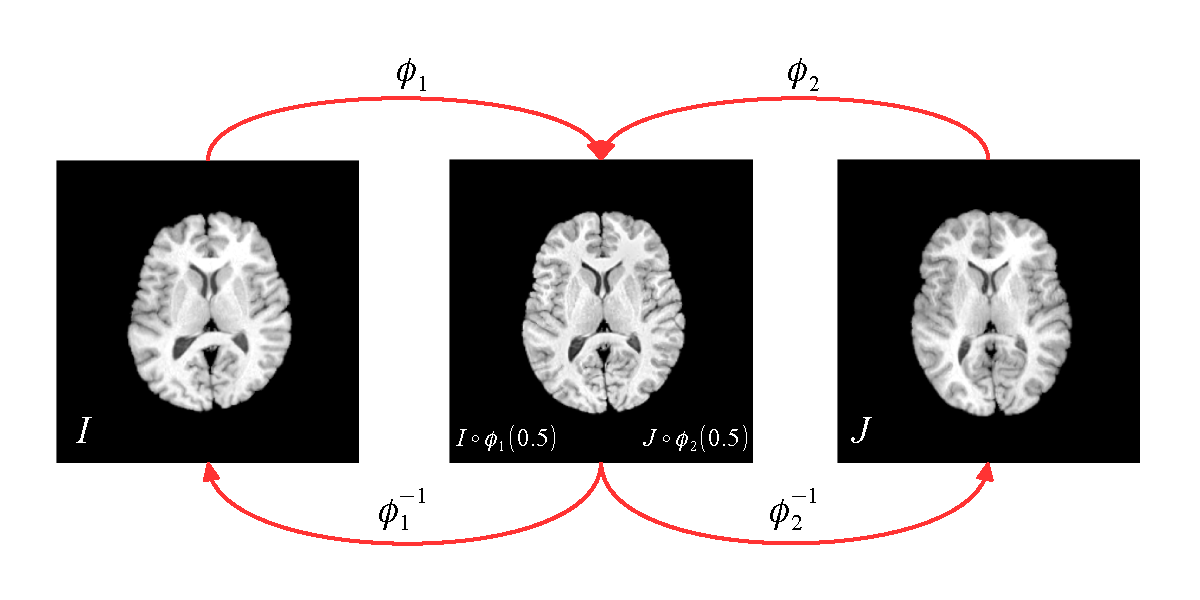
\includegraphics[width=0.95\textwidth]{SyN.pdf}
  \caption{Illustration of the greedy SyN formulation.  Given images
  $I_A$ and $I_B$, the symmetric set-up requires finding the two
  transform pairs $\left(\phi_1,\phi_1^{-1}\right)$
  $\left(\phi_2,\phi_2^{-1}\right)$ which map to/from
  the respective images to the midway point. During
  optimization, the update field at each iteration is
  determined from the metric field gradient taken at
  the midway point, i.e.
  $\nabla \Pi_{\sim} \left(I\circ\phi_1(0.5),J\circ\phi_2(0.5)\right)$.
  The full
  forward and inverse transforms are found through
  composition, i.e. $\phi=\phi_1 \circ \phi_2^{-1}$ and
  $\phi^{-1}=\phi_2 \circ \phi_1^{-1}$.
  }
  \label{fig:syn}
\end{figure}

\subsubsection{St. Nava's Theory of Greed and Original SyN}

Although presenting a rigorous framework for image registration solutions
with desirable properties, the complexity of these diffeomorphic methodologies
requires substantial computational resources.  For typical 3-D neuroimaging
applications, the corresponding solutions require numerical integration over
and storage of 4-D velocity fields at each iteration which is limiting for
many common, contemporary processing infrastructures.

Therefore, in addition to the full-scale
symmetric SyN offering described in \cite{avants2008}, the authors therein
provided a ``greedy'' alternative which has demonstrated superior performance
in various applications \citep{avants2011,klein2009,murphy2011}%
\footnote{
SyN was also the standard registration for the MICCAI 2013
Workshop on Segmentation:  Algorithms Theory, and Applications (SATA)
and corresponding challenge (https://masi.vuse.vanderbilt.edu/workshop2013).
}
while simultaneously being capable of running with limited computational
resources.  This is possible since the discrete time-parameterized
velocity field samples are restricted to their respective
endpoints, i.e. the $v_i(\mathbf{x},t)$ are sampled at $t \in \{0,0.5,1\}$
implying simultaneous storage of only four transform vector fields
$\phi_1(\mathbf{x})$,
$\phi_1^{-1}(\mathbf{x})$, $\phi_2(\mathbf{x})$, and $\phi_2^{-1}(\mathbf{x})$
(cf Figure \ref{fig:syn}).  Since the greedy SyN framework is the focus of the evaluation,
the algorithmic steps are briefly sketched
in Algorithm \ref{alg:syn}.

\begin{algorithm}
\caption{Greedy SyN algorithm}
\label{alg:syn}
\begin{algorithmic}
\State $\phi_i \leftarrow \mathbf{Id}$, $\phi_i^{-1} \leftarrow \mathbf{Id}$
\Comment $i \in \{1,2\}$
\State $n \leftarrow 1$
\While {not converged}
  \State $v_1^n \leftarrow \nabla \Pi_{\sim} \left(I\circ\phi_1^{n-1},J\circ\phi_2^{n-1}\right)$
  \State $v_2^n \leftarrow \nabla \Pi_{\sim} \left(J\circ\phi_2^{n-1},I\circ\phi_1^{n-1}\right)$
  \State $v_i^n \leftarrow S_v( v_i^n )$      \Comment $S_v$ is a smoothing operation on the update transform field
  \State $\phi_i^n \leftarrow S_\phi( v_i^n \circ \phi_i^{n-1} )$      \Comment $S_\phi$ is a smoothing operation on the total transform field
  \State $\left(\phi_i^n\right)^{-1} \leftarrow Inv\left(\phi_i^n, \left(\phi_i^{n-1}\right)^{-1}\right)$
    \Comment Inverse field estimation described in \cite{avants2008}
  \State $n \leftarrow n + 1$
\EndWhile
\State \Return $\phi \leftarrow \phi_1 \circ \phi_2^{-1}$, $\phi^{-1} \leftarrow \phi_2 \circ \phi_1^{-1}$
\end{algorithmic}
\end{algorithm}


\subsubsection{Directly Manipulated Free-Form Deformation Diffeomorphic Analogs}

Although several velocity field regularization
operators have been proposed, many algorithmic instantiations
default to Gaussian smoothing due to its simplicity both in implementation
and complexity terms.  As mentioned earlier, 
a viable and practical alternative is the DMFFD 
approach based on B-splines for explicit regularization of vector fields.
As presented in \cite{tustison2009}, given the similarity metric
$\Pi_{\sim}$, the $d$-dimensional update field (i.e. preconditioned
gradient field), $\delta v_{i_1,\ldots,i_d}$, is calculated from
\begin{align}
\label{eq:dmffd}
  \delta v_{i_1,\ldots,i_d} = \frac{ \sum_{c=1}^{N_{\Omega}} \left( \frac{\partial \Pi_\sim}{\partial \mathbf{x}} \right)_c \prod_{j=1}^d B_{i_j}(x_j^c)  
  \cdot \frac{\prod_{j=1}^d B_{i_j}^2 (x_j^c)}
  {\sum_{k_1=1}^{r+1}\ldots\sum_{k_d=1}^{r+1} 
  \prod_{j=1}^d B_{k_j}^2 (x_j^c)} }
  {\sum_{c=1}^{N_{\Omega}} \prod_{j=1}^d B_{i_j}^2 (x_j^c)}
\end{align}
where the set of $B(\cdot)$ are the univariate B-spline basis functions for
separately modulating regularity in the solution for each parametric dimension,
$N_\Omega$ is the number of voxels in the reference image domain,
$r$ is the spline order in all dimensions,%
\footnote{
In terms of implementation spline orders can be specified separately for each dimension but, for simplicity,
we only specify a single spline order.
}
and $\frac{\partial \Pi_\sim}{\partial \mathbf{x}}$ is the spatial 
similarity metric gradient indexed by $c$.

Similarly, in the case of $d$-dimensional time-parameterized 
diffeomorphic image registration, 
the time-dependent velocity field can be represented
as a $(d + 1)$-dimensional B-spline object
\begin{align}
v(\mathbf{x}, t) = \sum_{i_1=1}^{X_1}\ldots\sum_{i_d=1}^{X_d}\sum_{i_t=1}^T v_{i_1,\ldots,i_d,i_t} B_{i_t}(t) \prod_{j=1}^d B_{i_j}(x_j)
\end{align}
where $v_{i_1,\ldots,i_d,i_t}$ is a $(d+1)$-dimensional control point lattice
characterizing the velocity field.  The preconditioned gradient analog of
Equation (\ref{eq:dmffd}) for updating the time-varying velocity field control point lattice is 
\begin{align}
\label{eq:tvdmffd}
  \delta v_{i_1,\ldots,i_d,i_t} &= \left( \sum_{c=1}^{N_{\Omega} \times N_t} \left( \frac{\partial \Pi_\sim}{\partial \mathbf{x}} \right)_c B_{i_t}(t^c)\prod_{j=1}^d B_{i_j}(x_j^c)  \right. \nonumber \\
  &\cdot \left. \frac{B_{i_t}^2(t^c) \prod_{j=1}^d B_{i_j}^2 (x_j^c)}
  {\sum_{k_1=1}^{r+1}\ldots\sum_{k_d=1}^{r+1} \sum_{k_t=1}^{r+1} B_{k_t}^2(t^c)
  \prod_{j=1}^d B_{k_j}^2 (x_j^c)} \right) \nonumber \\
  &\cdot\left({\sum_{c=1}^{N_{\Omega}\times N_t}B_{i_t}^2(t^c) \prod_{j=1}^d B_{i_j}^2 (x_j^c)} \right) ^{-1}
\end{align}
which takes into account the temporal locations of the
dense gradient field sampled in $t \in [0,1]$. $N_t$ and $N_\Omega$ are the number
of time point samples and the number of voxels in the reference image domain, respectively.
\footnote{
Additionally, in \cite{tustison2006} it was shown that one could associate each
a sample, $\left( \frac{\partial \Pi}{\partial \mathbf{x}}\right)_c$ with a confidence
weighting.  Thus, in order to enforce stationary boundaries for all described
DMFFD-based diffeomorphic algorithms, we
assign image boundary metric gradients a value of zero with a corresponding
large confidence value.
}

For regularization of constant velocity fields, e.g. SyN or DARTEL, updating the 
field is performed using Equation (\ref{eq:dmffd}).  In the case B-spline SyN, 
this applies to the smoothing operators $S_{v}$ and $S_{\phi}$ in Algorithm \ref{alg:syn}
although best performance (at least for the data described in this work) typically
employs no smoothing on the total transform field, i.e. $S_\phi$ is such that $S_\phi( \phi_i^n ) = \phi_i^n$.



\subsection{Implementation}

Three diffeomorphic algorithms described previously utilizing Gaussian convolution smoothing and their DMFFD counterparts are available through the following classes in the ITK repository: 
\begin{itemize}
  \item {\bf LDDMM:}
    \begin{itemize}
      \item {\tt itk::TimeVaryingVelocityFieldTransform} 
      \item {\tt itk::TimeVaryingVelocityFieldTransformParametersAdaptor}
      \item {\tt itk::TimeVaryingVelocityFieldImageRegistrationMethodv4}
      \item {\tt itk::GaussianSmoothingOnUpdateTimeVaryingVelocityFieldTransform}
      \item {\tt itk::TimeVaryingBSplineVelocityFieldTransform} 
      \item {\tt itk::TimeVaryingBSplineVelocityFieldImageRegistrationMethodv4}
      \item {\tt itk::TimeVaryingBSplineVelocityFieldTransformParametersAdaptor}
    \end{itemize}  
  \item {\bf DARTEL:}
    \begin{itemize}
       \item{\tt itk::ConstantVelocityFieldTransform}
       \item{\tt itk::ConstantVelocityFieldTransformParametersAdaptor}
      \item {\tt itk::GaussianExponentialDiffeomorphicTransform} 
      \item {\tt itk::GaussianExponentialDiffeomorphicTransformParametersAdaptor}
      \item {\tt itk::BSplineExponentialDiffeomorphicTransform} 
      \item {\tt itk::BSplineExponentialDiffeomorphicTransformParametersAdaptor}
    \end{itemize}  
  \item {\bf SyN:}
    \begin{itemize}
      \item {\tt itk::SyNImageRegistrationMethod} 
      \item {\tt itk::BSplineSyNImageRegistrationMethod} 
    \end{itemize}  
\end{itemize}
These and other classes (e.g. similarity metrics, optimization methods, and
utility classes) were developed as part of the ITKv4 registration
framework refactoring.  Further details can be found in the documentation
provided within the classes themselves.%
\footnote{
http://www.itk.org/Doxygen/html/classes.html
}

The class {\tt itk::BSplineScatteredDataPointSetToImageFilter} underlies all DMFFD regularization which is an implementation of the 
methods described in \cite{tustison2006}.  Although applicable to
various scenarios (e.g. curve and surface estimation), it has
been optimized for imaging applications and multi-threaded
for fast processing on suitable machines.
Additionally, numerical integration for solving Equations (\ref{eq:ode}) and (\ref{eq:integral}) utilizes Runge-Kutta which
provides a more stable alternative than other
methods \citep{press2007}.  Implementation is provided in the class {\tt itk::TimeVaryingVelocityFieldIntegrationImageFilter}.

A complete packaging of these classes has been made
available as part of our Advanced Normalization Tools (ANTs) toolkit.%
\footnote{
http://stnava.github.io/ANTs/
}
The \verb#antsRegistration# program%
\footnote{
The long and short command line help menus can be invoked by
the commands `{\tt antsRegistration --help}' and `{\tt antsRegistration -h}', respectively.
}
takes advantage of the enhanced ITKv4
registration framework and was developed by the 
authors to provide a robust and versatile solution for a wide variety of
image registration applications. The basic conceptualization for use is that one 
can
set-up any number of registration ``stages'' with each stage being 
characterized by a specified transform.  For example, a representative 
command call is as follows:
\vspace{2mm}
\lstset{frame = htb,
        framerule = 0.25pt,
        float,
        fontadjust,
        backgroundcolor={\color{listlightgray}},
        basicstyle = {\ttfamily\scriptsize},
        keywordstyle = {\ttfamily\color{listkeyword}\textbf},
        identifierstyle = {\ttfamily},
        commentstyle = {\ttfamily\color{listcomment}\textit},
        stringstyle = {\ttfamily},
        showstringspaces = false,
        showtabs = false
        numbers = none,
        numbersep = 6pt,
        numberstyle={\ttfamily\color{listnumbers}},
        tabsize = 2,
        language=bash,
        floatplacement=!h,
        caption={Representative script containing {\tt antsRegistration} and {\tt antsApplyTransforms} command calls used for evaluation},
        captionpos=b,
        label=listing:script
        }
\begin{lstlisting}
# Register the $fixed and $moving images with initial
# alignment of the centers of intensity followed by 
# the following three stages:
#   rigid -> affine -> B-spline SyN

antsRegistration --dimensionality 3 \
                 --output ${prefix} \
                 --use-histogram-matching 1 \
                 --initial-moving-transform [${fixed},${moving},1] \
                 --transform Rigid[0.1] \
                 --metric MI[${fixed},${moving},1,32,Regular,0.25] \ 
                 --convergence 1000x500x250 \
                 --smoothing-sigmas 2.0x1.0x0.0mm \
                 --shrink-factors 4x3x2 \
                 --transform Affine[0.1] \
                 --metric MI[${fixed},${moving},1,32,Regular,0.25] \ 
                 --convergence 1000x500x250 \
                 --smoothing-sigmas 2.0x1.0x0.0mm \
                 --shrink-factors 4x3x2 \
                 --transform BSplineSyN[0.1,26,0x0x0,3] \
                 --metric CC[${fixed},${moving},1,4] \ 
                 --convergence 100x70x50x20 \
                 --smoothing-sigmas 2x1.0x0.5x0.0mm \
                 --shrink-factors 6x4x2x1

# Apply the resulting transforms (generic affine + 
# B-spline SyN) to the moving labels.
                   
antsApplyTransforms --dimensionality 3 \
                    --input ${moving_labels} \
                    --reference-image ${fixed} \
                    --output ${moving_warped_labels} \
                    --n NearestNeighbor \
                    --transform ${prefix}1Warp.nii.gz \
                    --transform ${prefix}0GenericAffine.mat \
                    --default-value 0
\end{lstlisting}
In this example, we first calculate an initial translation transform by aligning
the centers of (intensity) mass. The resulting transform is then used as input 
for determining an optimal rigid transform.  Serial propagation of the resulting
composite transform continues until all optimal transforms have been determined.
Optimization for each stage is determined by the specified general parameters 
including: smoothing and downsampling of fixed and moving images, convergence
criteria (including number of iterations per resolution level) and metric (or
metrics).  Note that any pair of images can be specified per stage.  

Although the
resulting transforms for each stage can be written to disk as output, the 
default output consists of a condensed set of transforms where compatible 
transforms have been composed to a single transform.  For example, in the
above command call, the initial translation, rigid, and affine transforms are
combined into a single generic affine transform file with the results of the
deformable transform consisting of discrete vector fields.  The output
transform files can then be applied using the {\tt antsApplyTransforms}
program which permits composition of any number of transform files with 
various interpolation schemes.   For both programs interpolation is never
performed more than once. 


\subsection{Evaluation Data}

\begin{figure}[htb]
  \centering
  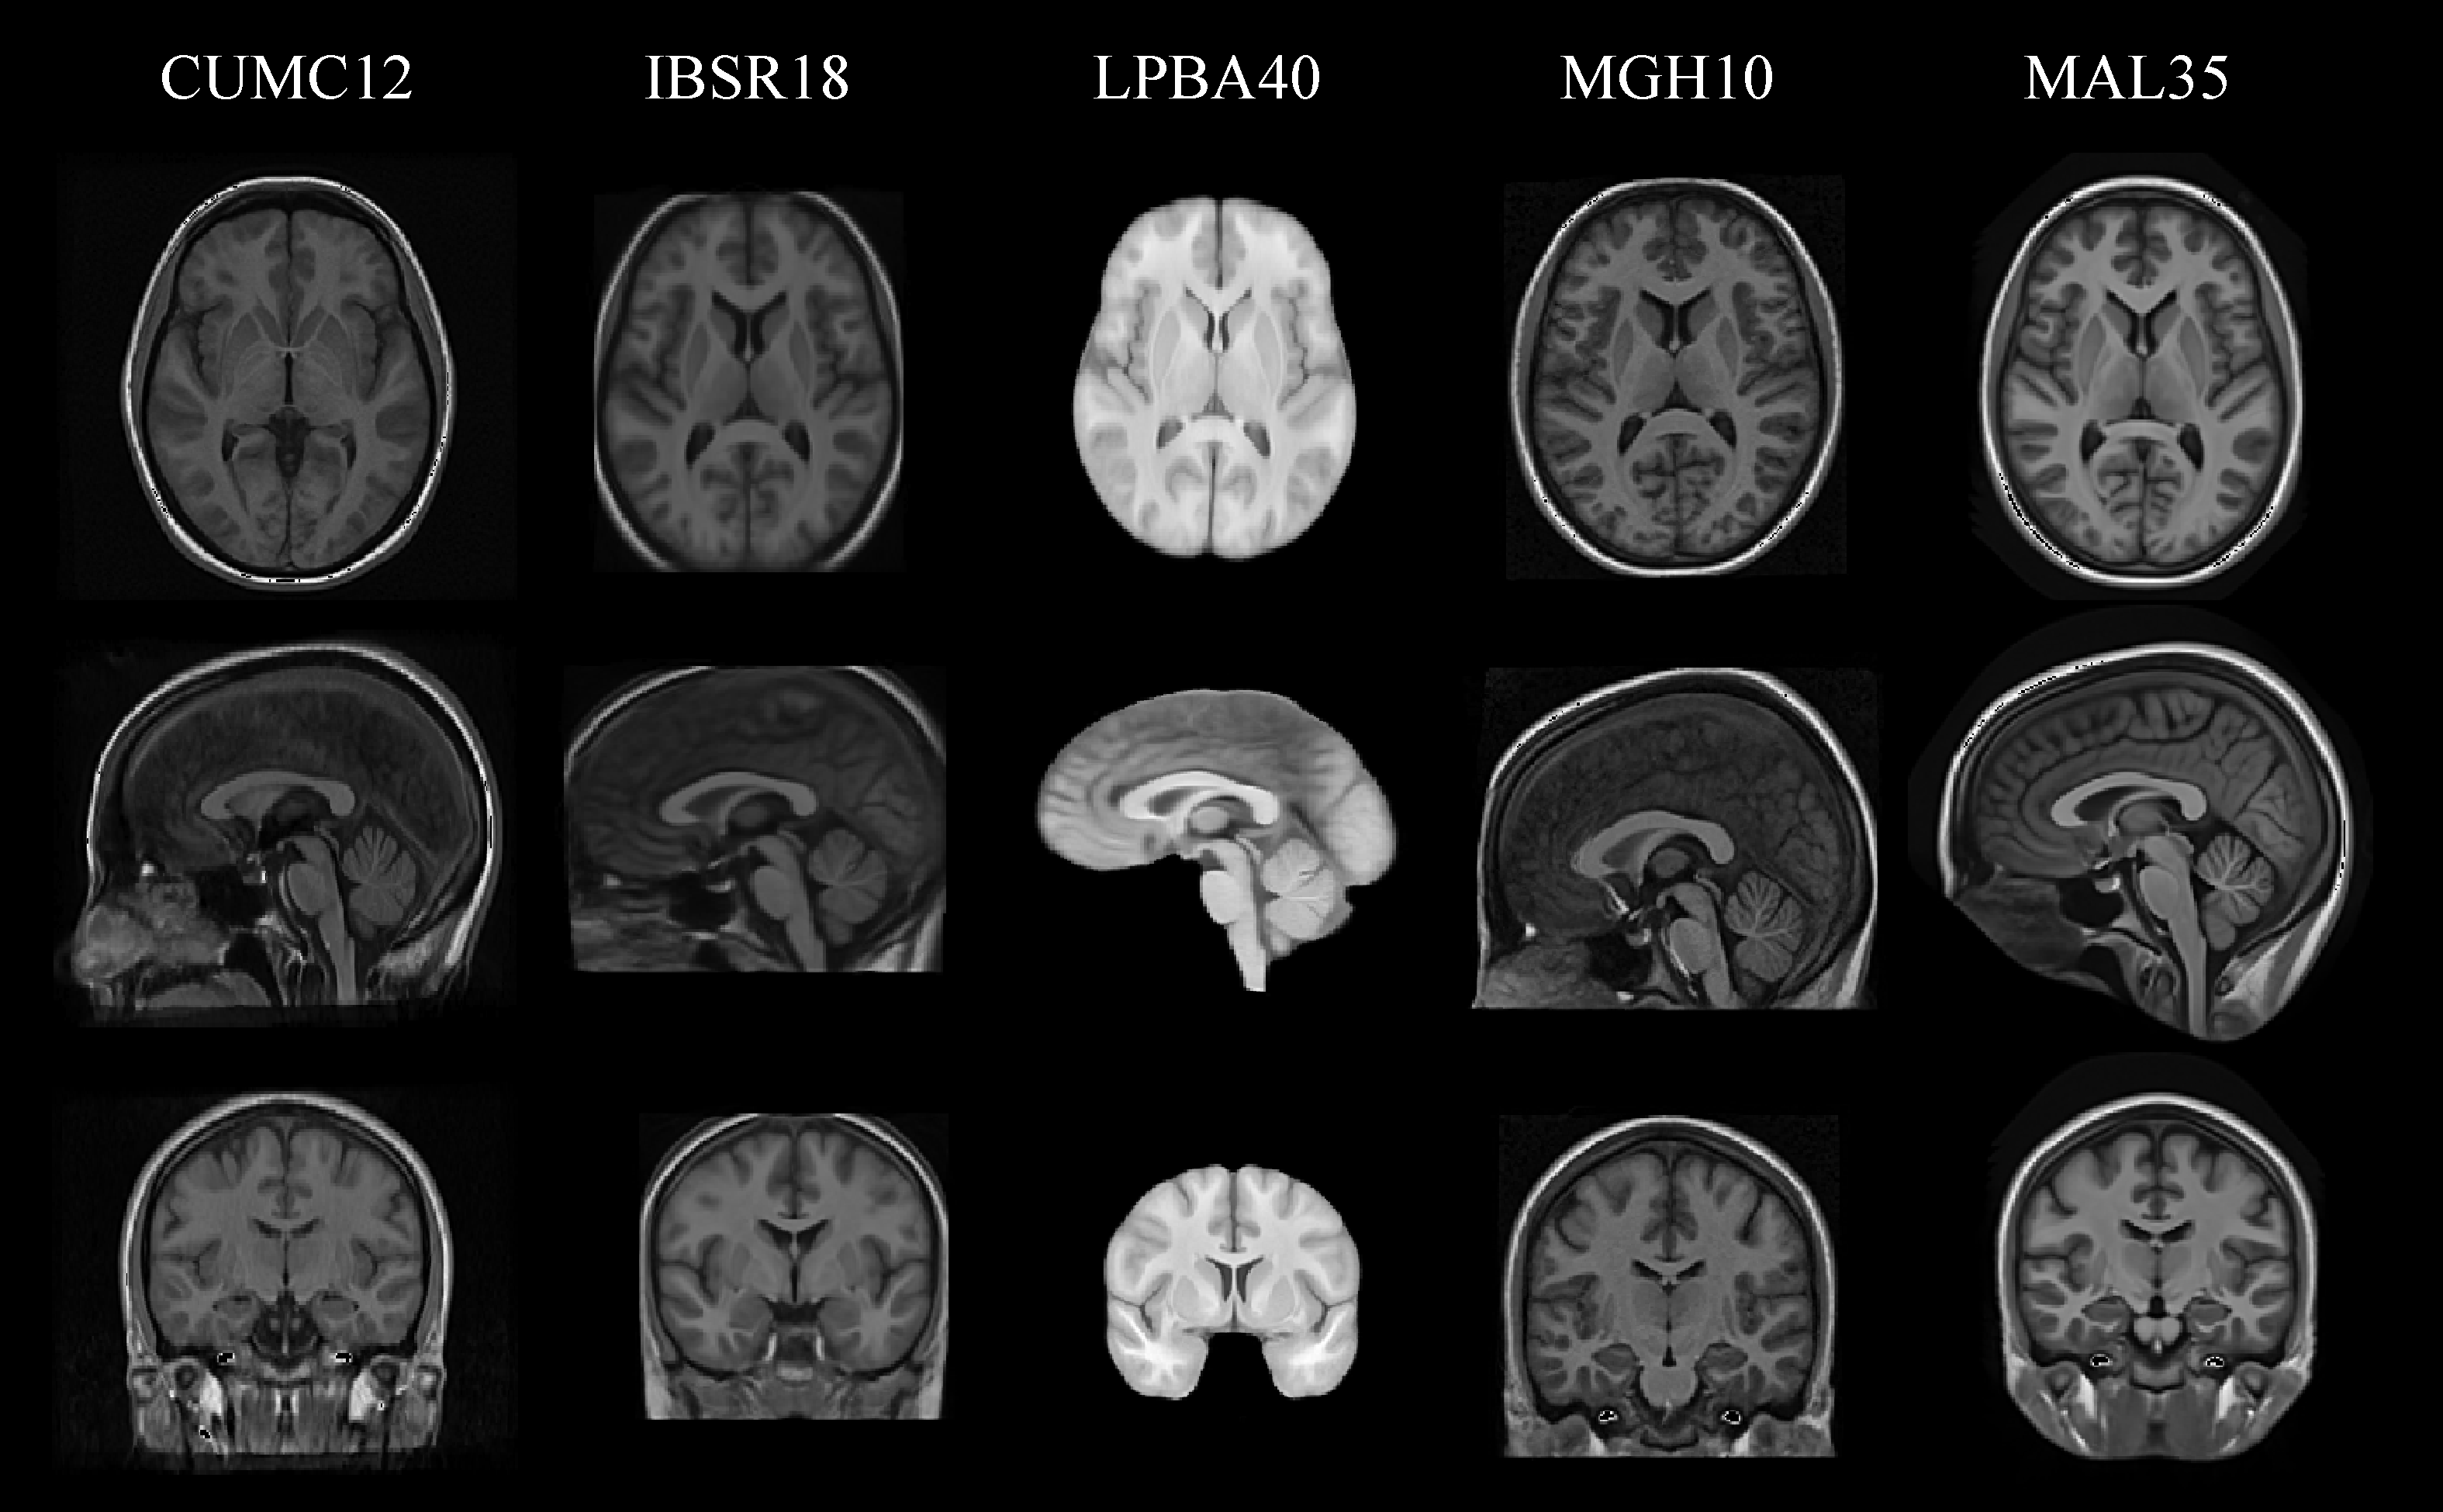
\includegraphics[width=0.95\textwidth]{templates.pdf}
  \caption{Canonical views for each of the five cohort-specific templates generated using
  the ANTs tools as described
  in \cite{avants2010}.   The pseudo-geodesic transform between subjects is created from 
  the composition of transforms to/from the relevant template.
  }
  \label{fig:templates}
\end{figure}

In the well-known Klein comparative study \citep{klein2009}, 14 image registration
algorithms were evaluated based on performance on publicly available labeled brain data.
%Based on the final rankings, the SyN algorithm was determined to be one
%of the top-performing deformable registration algorithms.  Its relative
%performance coupled with its public availability has made
%it a de facto standard for algorithmic comparison.
For our evaluation, we used these same data.  
Specifically, we used the data sets denoted as:
\begin{itemize}
  \item MGH10 
  \item CUMC12
  \item IBSR18
  \item LPBA40
\end{itemize}
which are available for download from Arno Klein's website.%
\footnote{
http://mindboggle.info/papers/evaluation\_NeuroImage2009.php
}
The number of subjects per cohort is provided in the denotation.
Further details of these labeled brain data (e.g. labeling protocol,
data sources) are given in \citep{klein2009}.
We also include the labeled brain data provided at the
MICCAI 2012 Grand Challenge and Workshop on Multi-Atlas
Labeling%
\footnote{
https://masi.vuse.vanderbilt.edu/workshop2012
} 
which we denote as MAL35.  This T1-weighted
MRI data set consists of 35 subject MRIs taken from the
Oasis database.%
\footnote{
http://www.oasis-brains.org
}  The corresponding labels were provided by Neuromorphometrics,
Inc.%
\footnote{
http://Neuromorphometrics.com/
}
under academic subscription.

\begin{figure}[htb]
  \centering
  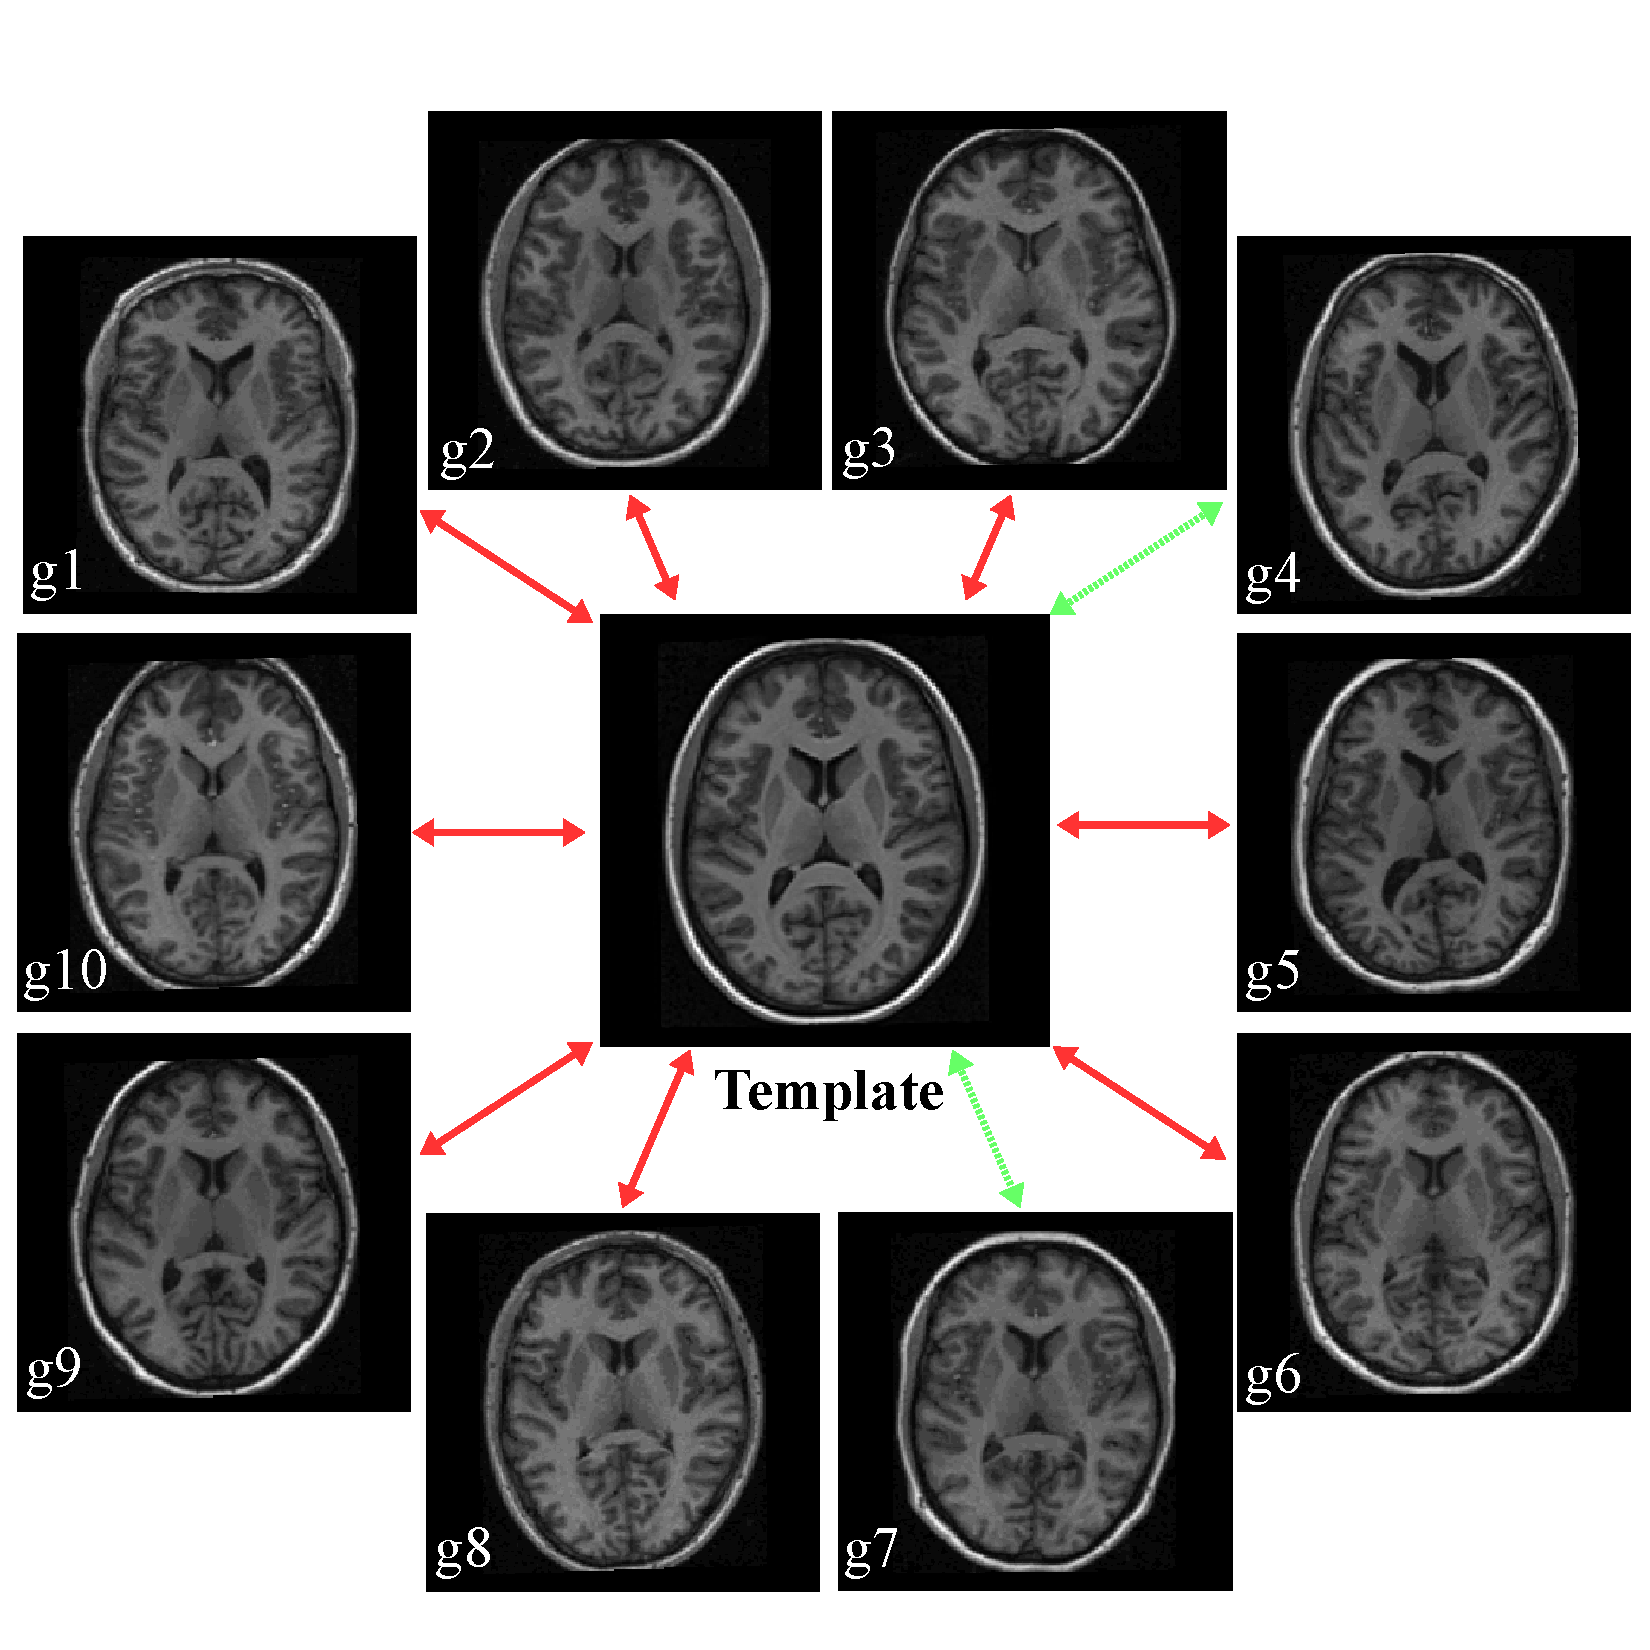
\includegraphics[width=0.75\textwidth]{pseudo_geodesic.pdf}
  \caption{Illustration of generating a pseudo-geodesic for any two subjects
  within the MGH10 cohort.  Once the transforms between the
  template and each subject are calculated, the mapping between any two
  subjects is found by composition of forward and inverse transforms.  For
  example, in the MGH data set, the pseudo-geodesic transform to
  map Subject g4 to Subject g7 is found by composing the forward
  transform from g4 to the template with the inverse transform from the
  template to g7 (green dashed lines).
  }
  \label{fig:pseudo_geodesic}
\end{figure}

Comparative evaluation of the two SyN registration approaches was performed 
within each cohort using a ``pseudo-geodesic'' approach.  Instead of
registering every subject to every other subject within a data set,
we generated the transforms from each subject to a cohort-specific
shape/intensity template.  This was accomplished using the ANTs script {\tt antsMultivariateTemplateConstruction.sh}
which is a multivariate implementation of the work described in
\cite{avants2010}. Canonical views for each of the five templates
used for this study are given in Figure \ref{fig:templates}.  
Since calculation of the transform from each subject to the template also
includes generation of the corresponding inverse transform, the total
transformation from a given subject to any other is determined from the composition
of transforms mapping through the template.  An example illustration of the
geodesic approach is given in Figure \ref{fig:pseudo_geodesic}.

\begin{figure}[htb]
  \centering
  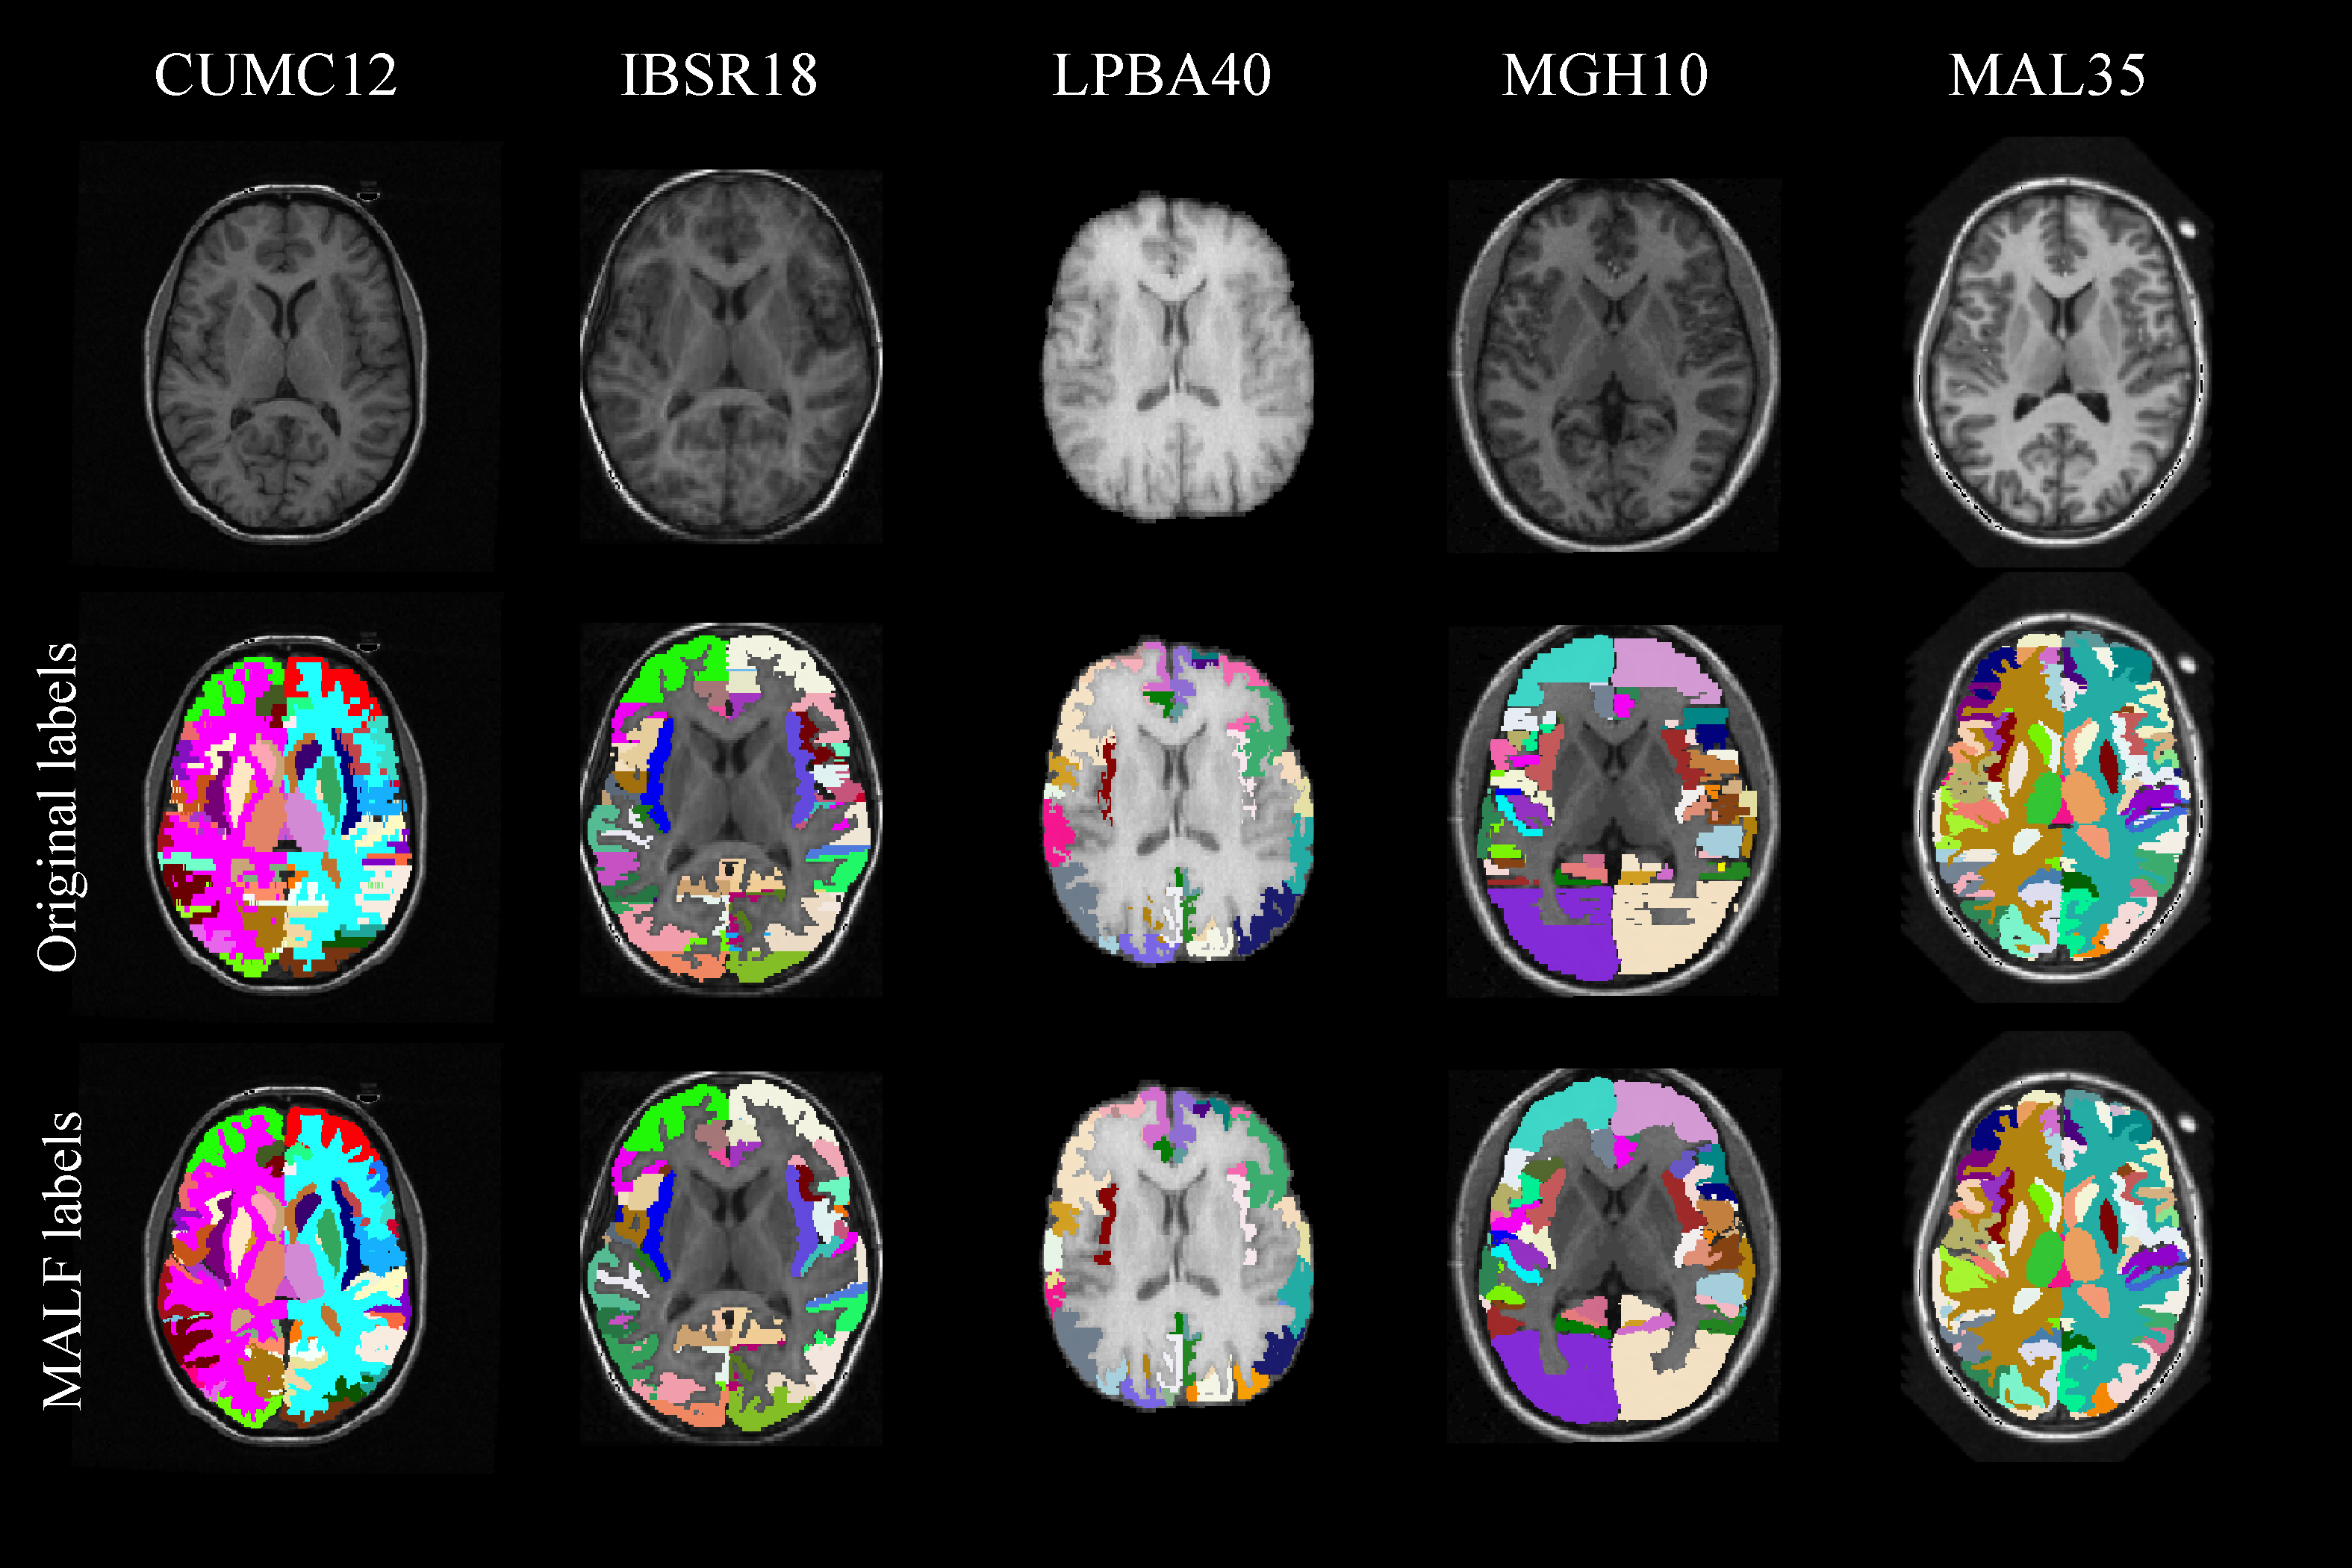
\includegraphics[width=0.95\textwidth]{labels.pdf}
  \caption{Axial views of sample labelings for a member of each data set.  
  The second row consists of the original labelings with the third row being
  refined versions of those labelings using the MALF algorithm \cite{wang2012}.
  These refinements provide more consistency between labelings and improved
  comparative assessments between algorithms.
  }
  \label{fig:labels}
\end{figure}

Additionally, we refined the labelings for each subject of each cohort
using the multi-atlas label fusion algorithm (MALF) developed by \cite{wang2012}
which is also distributed with the ANTs repository.
For a given subject within a data set, every other subject was mapped to 
that subject using the pseudo-geodesic transform.  The set of transformed labelings 
were then used to determine a consensus
labeling for that subject.
This was to minimize the obvious {\it observer dimensionality artifacts} where manual
raters observe and label in a single dimension at a time.  This
is most easily seen in the axial or sagittal views of the different cohorts 
as labelings were done primarily in the coronal view (see Figure \ref{fig:labels}).  
We include both sets of results.  This provides two sets of labels per subject
for evaluation.



\section{Results}
%Results should be clear and concise.

\begin{figure}[htb]
  \centering
  \begin{tabular}{ccccc}
  {} &
  \multicolumn{2}{c}{\bf Original labeling} & 
  \multicolumn{2}{c}{\bf MALF labeling} \\
  \rotatebox{90}{\qquad\,\, CUMC12} &
  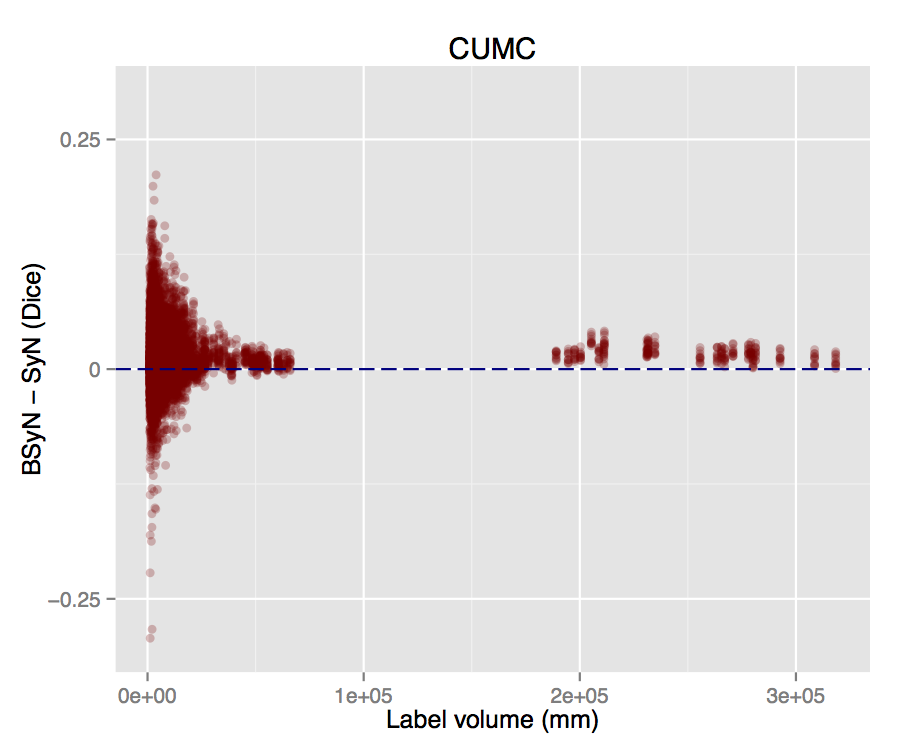
\includegraphics[height=38mm]{versusCUMC.png} &
  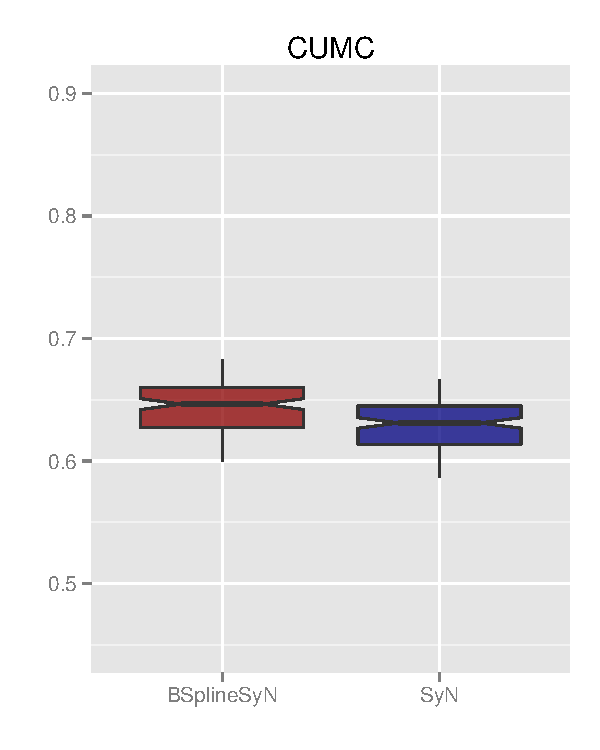
\includegraphics[height=38mm]{synComparisonCUMC.pdf} &
  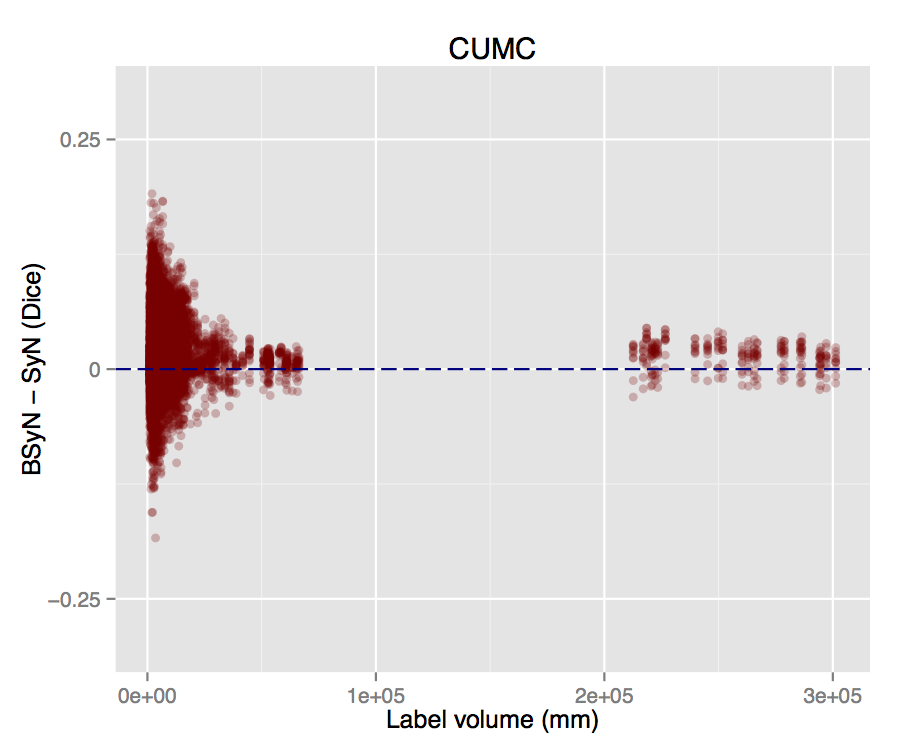
\includegraphics[height=38mm]{versusCUMCMALF.png} &
  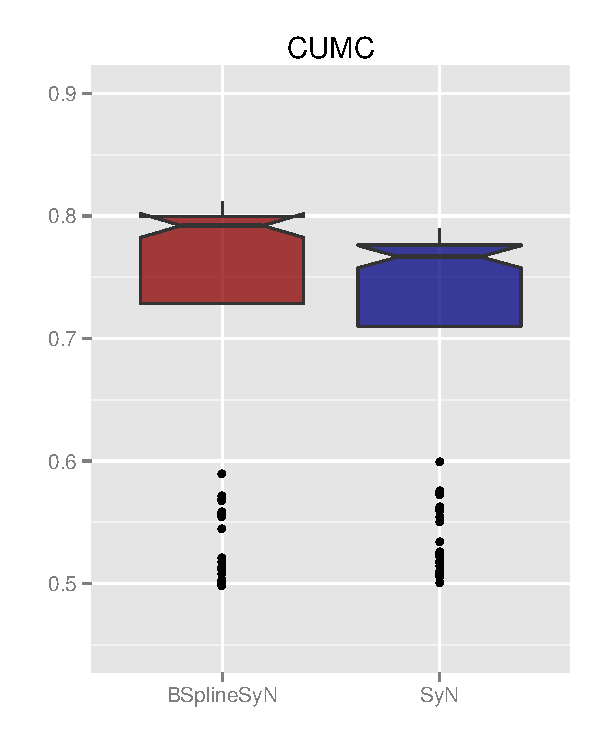
\includegraphics[height=38mm]{synComparisonCUMCMALF.pdf} \\
  \rotatebox{90}{\qquad\quad IBSR18} &
  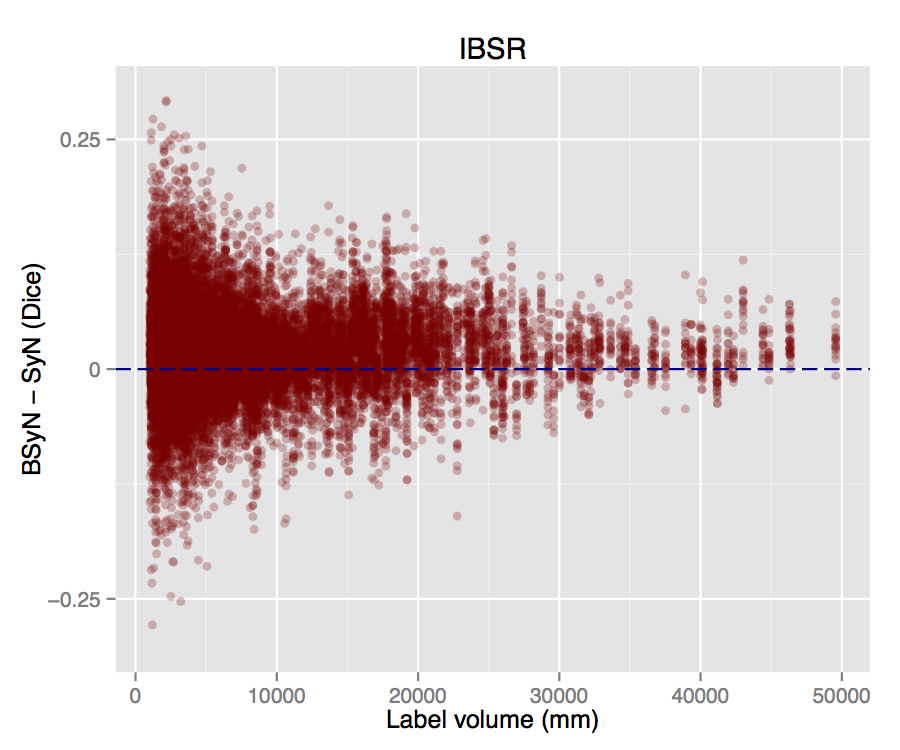
\includegraphics[height=38mm]{versusIBSR.png} &
  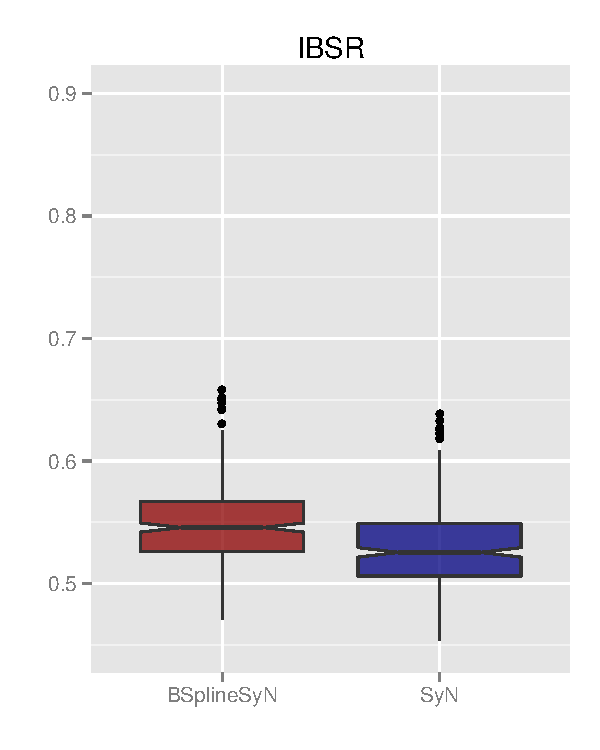
\includegraphics[height=38mm]{synComparisonIBSR.pdf} &
  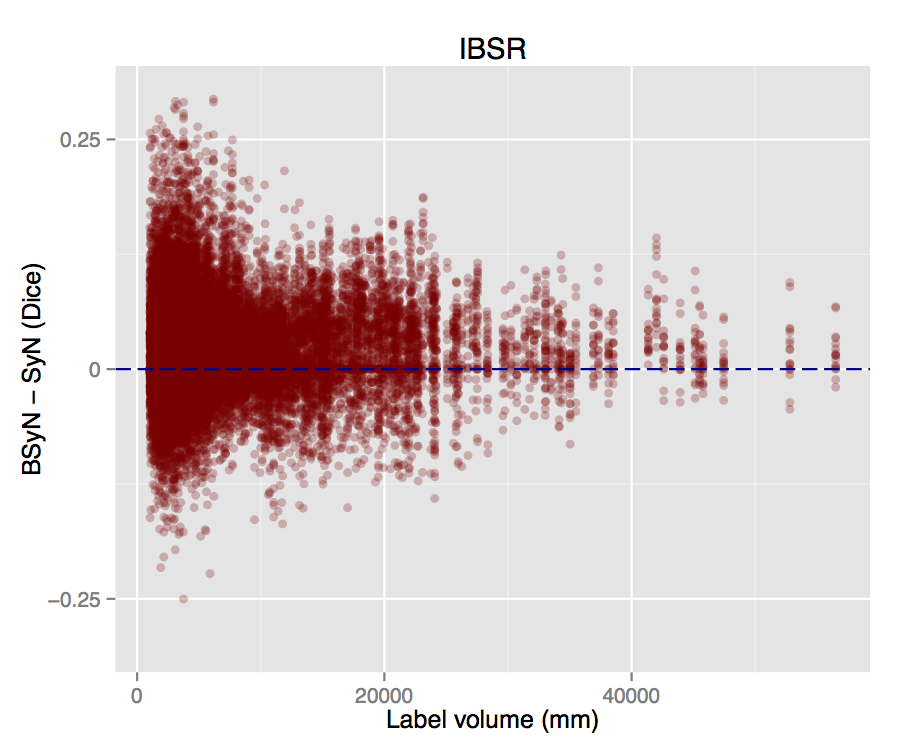
\includegraphics[height=38mm]{versusIBSRMALF.png} &
  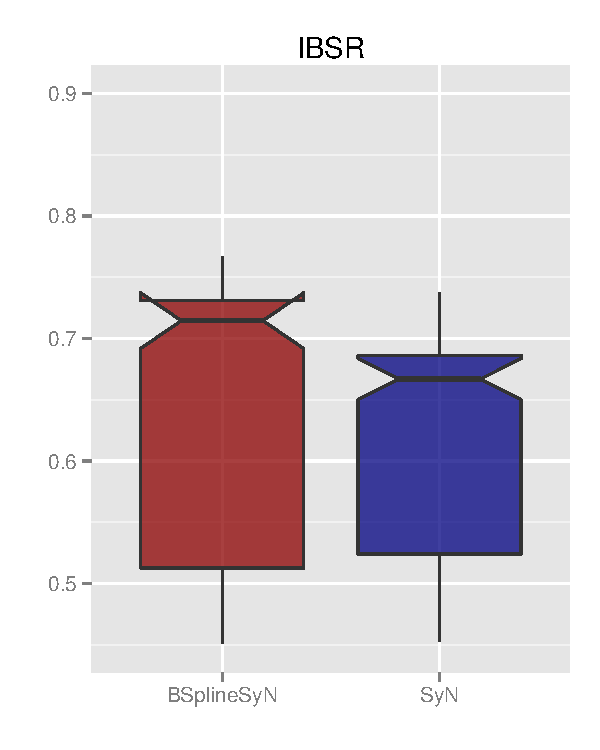
\includegraphics[height=38mm]{synComparisonIBSRMALF.pdf} \\
  \rotatebox{90}{\qquad\quad LPBA40} &
  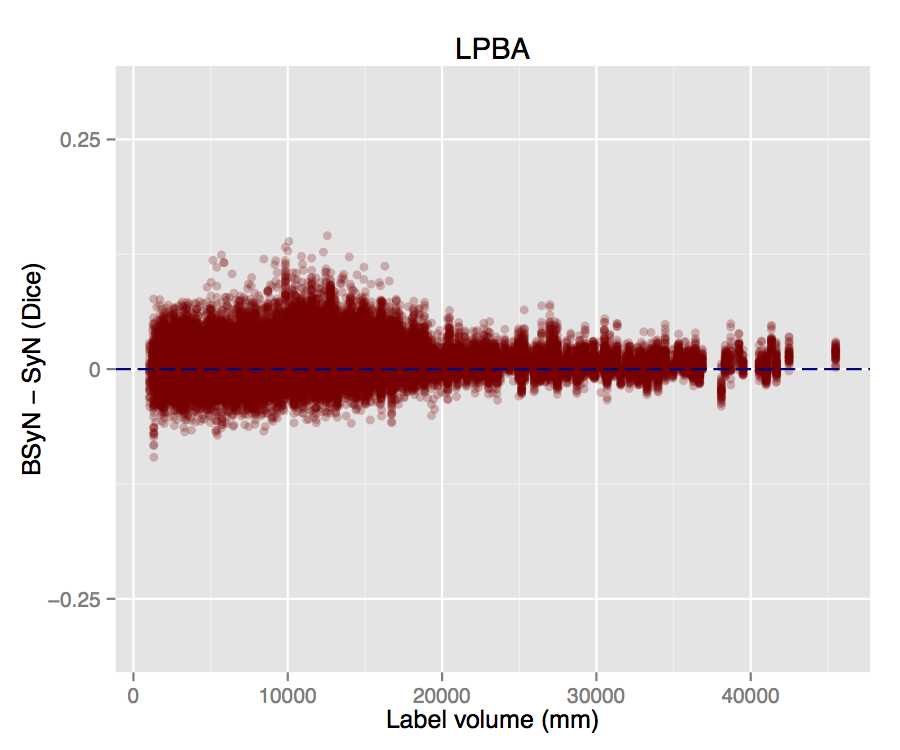
\includegraphics[height=38mm]{versusLPBA.png} &
  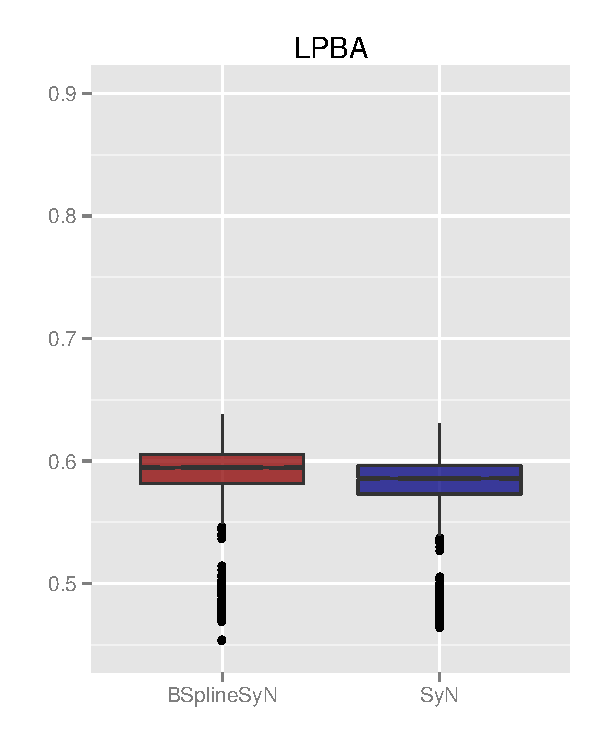
\includegraphics[height=38mm]{synComparisonLPBA.pdf} &
  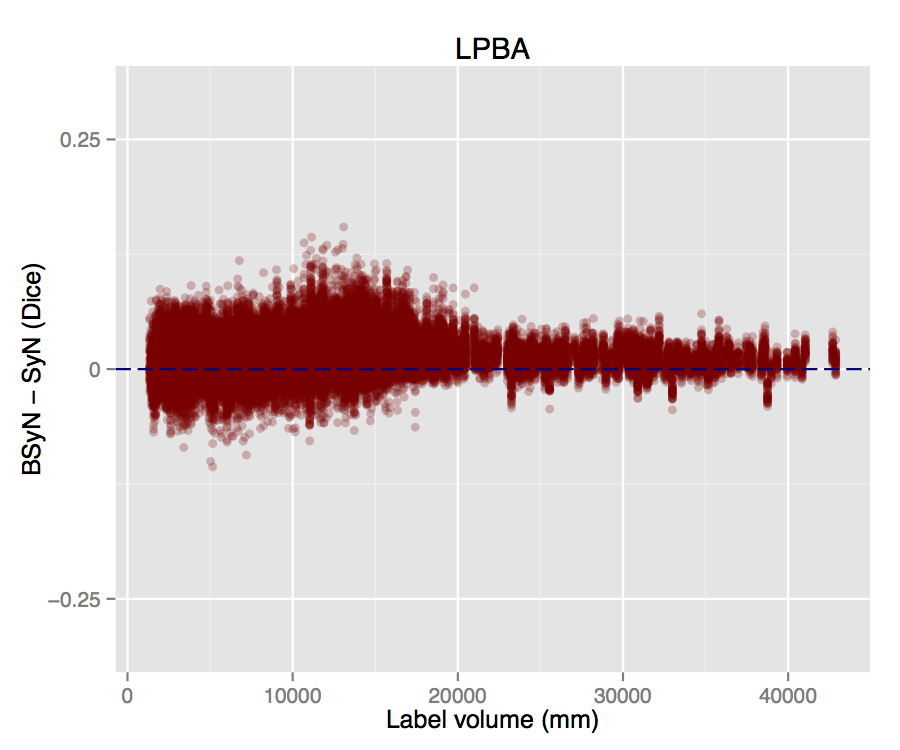
\includegraphics[height=38mm]{versusLPBAMALF.png} &
  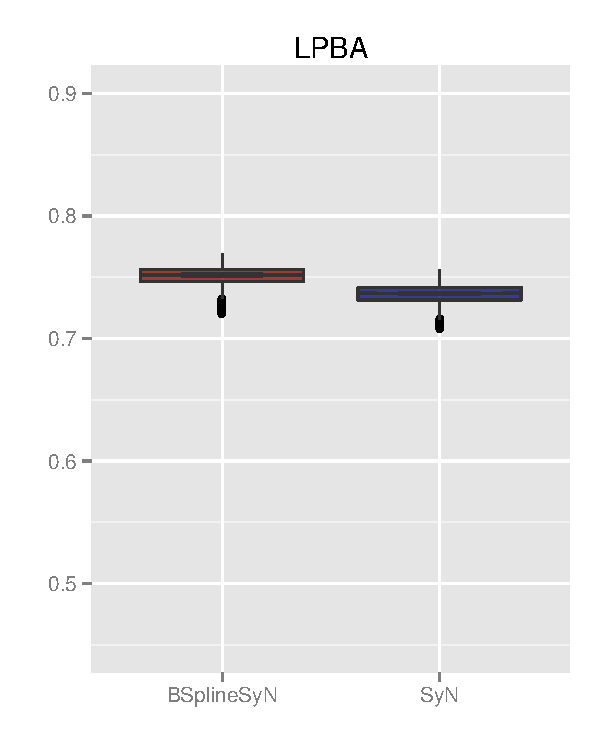
\includegraphics[height=38mm]{synComparisonLPBAMALF.pdf} \\
  \rotatebox{90}{\qquad\quad MGH10} &
  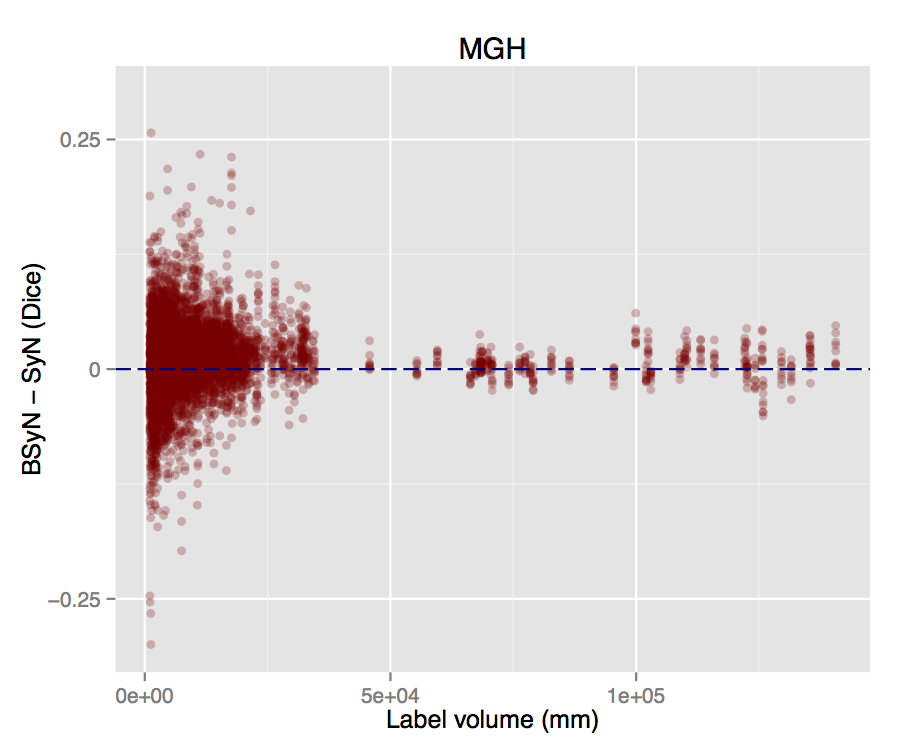
\includegraphics[height=38mm]{versusMGH.png} &
  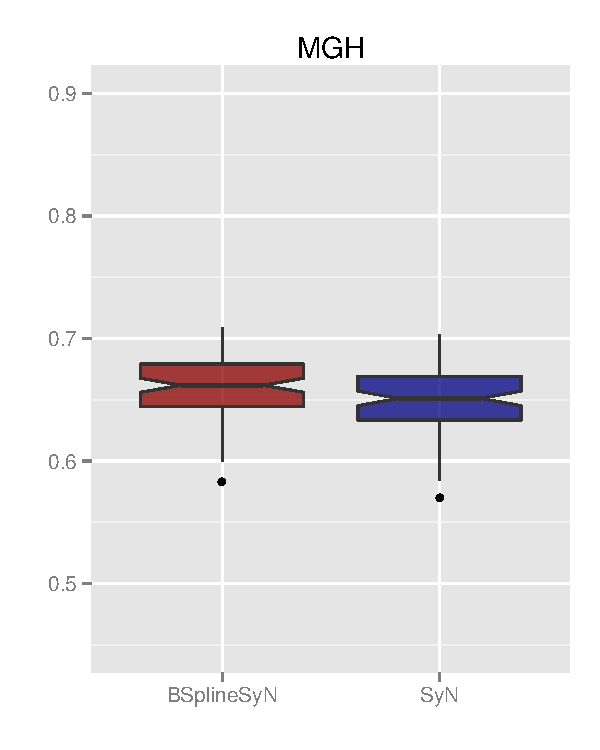
\includegraphics[height=38mm]{synComparisonMGH.pdf} &
  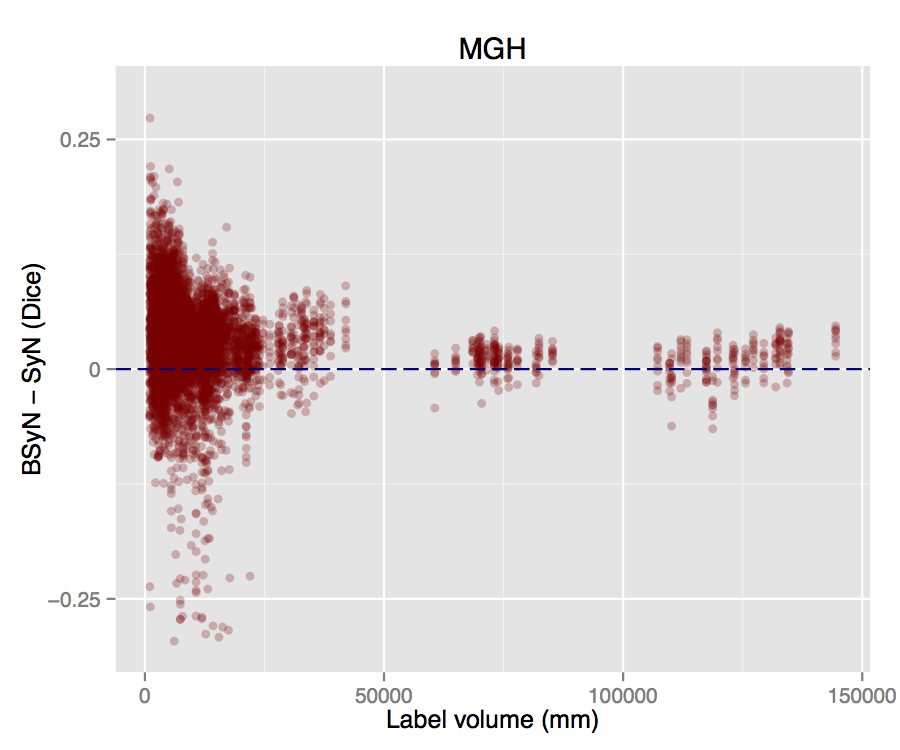
\includegraphics[height=38mm]{versusMGHMALF.png} &
  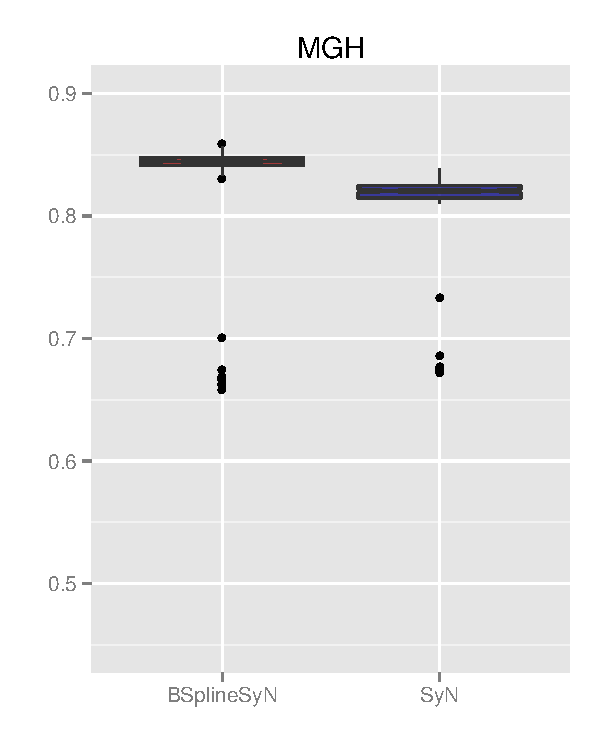
\includegraphics[height=38mm]{synComparisonMGHMALF.pdf} \\
  \rotatebox{90}{\qquad\quad MAL35} &
  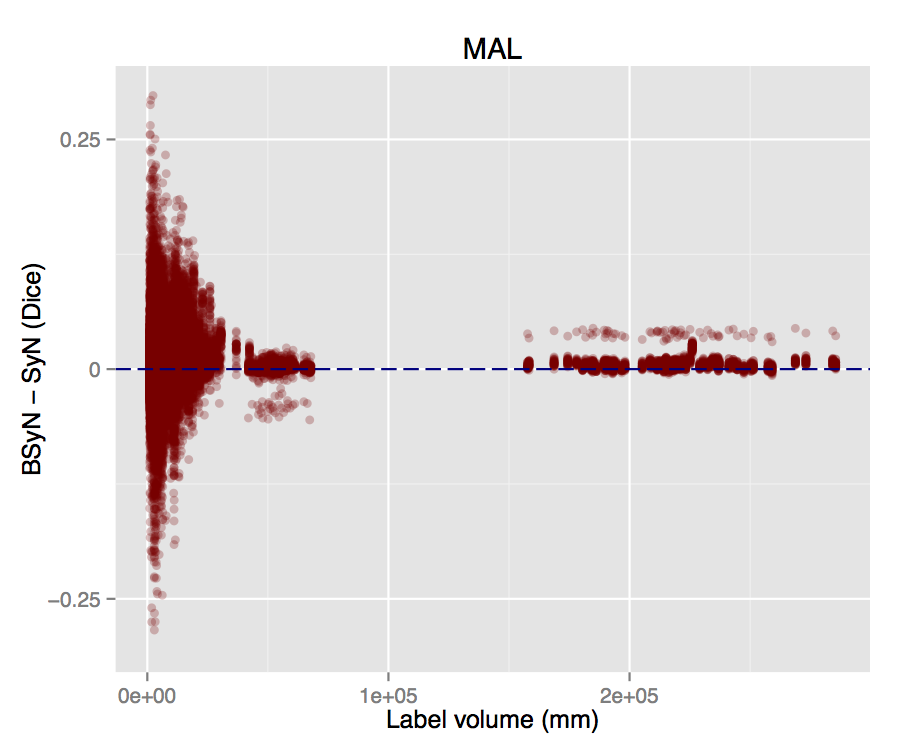
\includegraphics[height=38mm]{versusMAL.png} &
  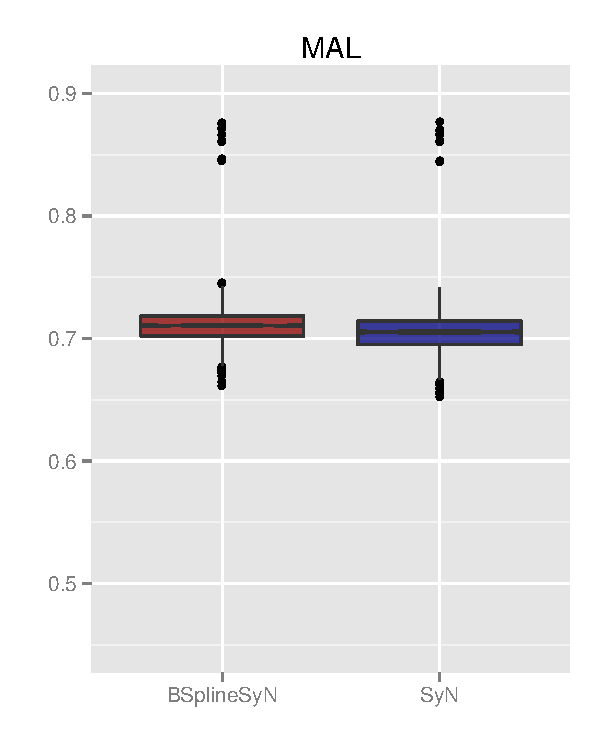
\includegraphics[height=38mm]{synComparisonMAL.pdf} &
  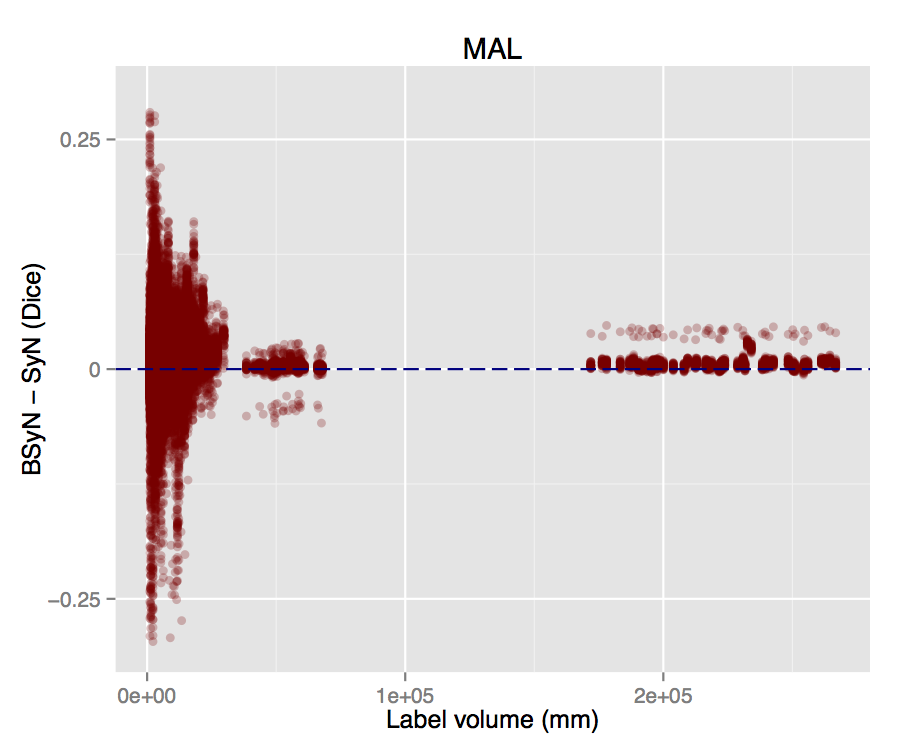
\includegraphics[height=38mm]{versusMALMALF.png} &
  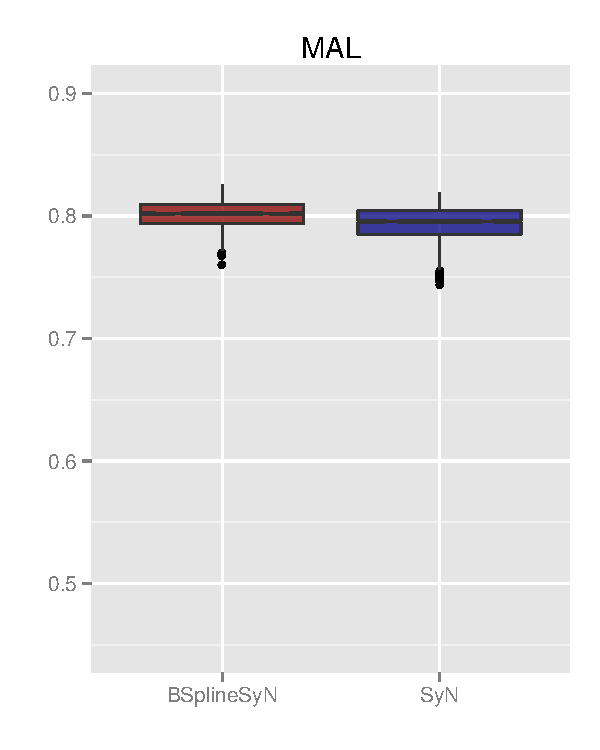
\includegraphics[height=38mm]{synComparisonMALMALF.pdf} \\
  \end{tabular}
  \caption{Dice results for both algorithms for 
  each subject warped to every other subject using the pseudo-
  geodesic transform.  Each 
  row corresponds to one of the five data sets used for evaluation.
  For each data set we include a plotting of all individual label 
  Dice results by volume and a combined label box plotting.  The
  left and right halves show the results for MALF-derived and 
  original labelings, respectively.
  }
  \label{fig:dice}
\end{figure}

As mentioned previously, a template was constructed for each data
set (cf Figure \ref{fig:templates}) from all cohort images.  Subsequently, 
each image was registered to its corresponding template using either 
SyN or B-spline SyN as described previously (prior linear registration 
stages were identical between the two algorithms).  As a brute-force parameter
exploration is not a part of this work, we rely on previously
reported research \citep{klein2009,avants2011} and our own experience as
authors/developers of the algorithm/software to select parameters which 
demonstrate robust performance across data sets.  For both algorithms,
the gradient step was 0.1 during each of the four multi-resolution levels
with shrink factors of $\{6,4,2,1\}$ with Gaussian smoothing for each
of those levels being $\mathcal{N}\left(0,\{9,4,1,0\}\right)$ in terms
of voxels.  The number of iterations per level were $\{100,100,70,20\}$
with a convergence threshold of $10^{-9}$ and window size of 15 iterations.

All processing was performed using the computational cluster at the 
University of Virginia.%
\footnote{
http://www.uvacse.virginia.edu
}
All perl scripts used to create the jobs for the cluster are
included in the github account associated with this evaluation.  
It should be noted that for the
data sets used in this study, times for B-spline SyN were approximately 
15-40\% greater than Gaussian-based SyN using single-threading and a dense
metric gradient sampling.

The differences between the two algorithms consist of the Gaussian and 
B-spline parameters governing the update field smoothing, $S_v$.  In our 
experience, smoothing of the total field did not improve the results, at
least for these data (which conforms with our experience with other
data), so the total field smoothing, $S_{\phi}$ is 0 for
both registration approaches.  Specifically, the chosen parameters
for the SyN algorithm were:  $S_{\phi} = \mathcal{N}(0,0)$ and 
$S_{v} = \mathcal{N}(0,3)$ in voxel terms.%
\footnote{
 Or, in equivalent {\tt antsRegistration} command line parlance, {\tt -t
 SyN[0.1,3,0]}.
 }  Although our experience with B-spline SyN is much more limited, we 
were able to choose comparable parameters based on a knot spacing
for the update field of 26 mm at the base level which is reduced by
a factor of two for each subsequent multiresolution level.  This 
yields a final knot spacing of 3.25 mm.%
\footnote{
 Or, equivalently, {\tt -t
 BSplineSyN[0.1,26,0]}.
% The {\tt antsRegistration} command line currently 
% permits specification of the
% B-spline total and update field smoothing only in terms of total mesh size over
% the entire image domain, i.e. {\tt -t BSplineSyN[0.1,10x10x8,0]}.  However, 
% in order to minimize anisotropic smoothing, we determined for each subject 
% the mesh size closest to producing a knot spacing of 26 mm which was typically
% around 10 mesh elements per dimension.  We are currently planning on modifying
% the command line to permit specification of a knot size (similar to the 
% ANTs-based N4 bias correction algorithm \citep{tustison2010} which also uses the
% same underlying B-spline computational machinery).
 }
As specified in the supplementary material associated with \cite{klein2009}, 
this is similar to the 
gradient smoothing parameter for the IRTK FFD algorithm
which also used four multi-resolution levels with an initial knot spacing of
20 mm per dimension for a final knot spacing of 2.5 mm.  

Quality of overlap  using the 
Dice similarity metric 
was determined from the transformed labels
using the open source ITK
implementation described in \cite{tustison2009a}.
Both the original labels and MALF labels were warped
to the fixed image for comparison using nearest neighbor
interpolation.  A joint Dice metric value was calculated
from the combined labels for each cohort for each of the
two SyN methods.  These values are rendered in notched
box plot format in Figure \ref{fig:dice}.  Non-overlapping notches
indicate approximately statistically significantly different median values
at the 95\% confidence level \citep{mcgill1978}.
For all data sets, the B-spline SyN variant showed a small but statistically
significant improvement in overall Dice values.
In order to provide a more complete picture of performance differences,
we also accounted for label volumetric considerations \citep{rohlfing2012}.  In Figure
\ref{fig:dice} we plotted the Dice value difference between each
SyN variant (B-spline SyN - SyN) for each label of each intra-subject
registration pair within a data set versus the volume of the label
in the fixed image.  

\begin{figure}[htb]
  \centering
    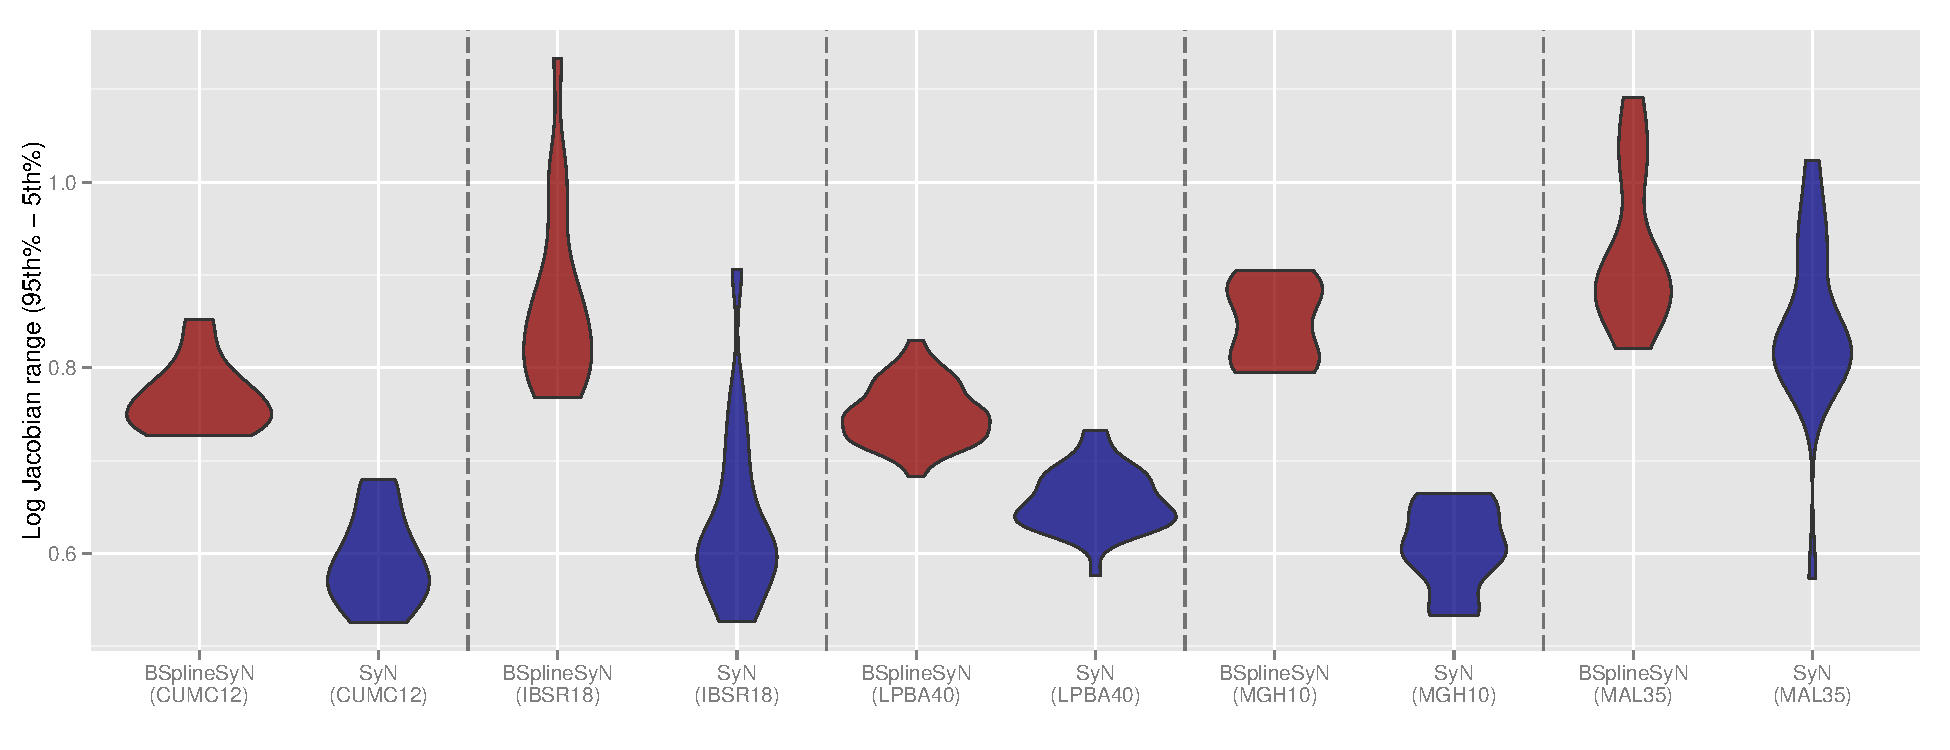
\includegraphics[width=0.95\textwidth]{jacobianRange.pdf}
  \caption{Violin plots of the range of log Jacobian values 
           (95th\% - the 5th\%)  
           for all deformable
           transforms from each subject to its corresponding
           template.  B-spline SyN demonstrates a tendency 
           to produce a much
           greater range of log Jacobian values.
           }
  \label{fig:jacobian}
\end{figure}

To further characterize the deformable transform differences, we 
calculated the log of the Jacobian determinant of the transformations from 
each subject to the template and 
tabulated statistical information within the brain region only. 
A noticeable difference between the two algorithms was the
respective range of values in log Jacobians.  We plotted the 
(95th\% - the 5th\%) for each algorithm across all data sets
 in Figure \ref{fig:jacobian}.  It is apparent 
that B-spline SyN produces a much greater range of deformation
values during the course of optimization.

\section{Discussion and Conclusions}
%This should explore the significance of the results of the work, not repeat them. A combined Results and Discussion section is often appropriate. Avoid extensive citations and discussion of published literature.

A significant amount of research has been devoted to image registration
algorithmic development.  Given their many salient characteristics particularly with
respect to large deformation estimation constrained by topological 
continuity, diffeomorphic registration
approaches have been a particular focus in the neuroimaging community.
However, many groups continue to find success with non-diffeomorphic
FFD methods
\citep[e.g.][]{rueckert1999,klein2010}.  Using our DMFFD framework, 
B-spline regularization is easily adapted into the diffeomorphic registration 
framework and performs comparably to analogous algorithms which we demonstrated 
in this work for the case of the widely-used SyN.

B-spline SyN produced slightly greater Dice values than the original SyN.
Interestingly it was shown that the range of log Jacobian values tend to be
significantly higher for the former than the latter.  Although possible 
explanations include the approximation-versus-convolution distinction mentioned
earlier, further exploration is planned.  


One of the advantages that has not been explored in this manuscript is 
the use of B-spline SyN for small deformation estimation problems such 
as in pulmonary or cardiac applications.  Such problems typically require
greater regularization which implies larger discrete Gaussian kernels.
A related issue is applications involving severely anisotropic data where
the continuous nature of the DMFFD approach might help over Gaussian convolution.
Additionally, we have not yet explored the use of sparsely sampled data 
and the advantages of the proposed framework.
Ongoing work will continue to explore these issues.


%Perhaps most important, in the spirt of open science, all source code
%used in this work is publicly available and well-vetted as part of the 
%ANTs initiative.  


%\section{Conclusions}
%The main conclusions of the study may be presented in a short Conclusions section, which may stand alone or form a subsection of a Discussion or Results and Discussion section.

%% The Appendices part is started with the command \appendix;
%% appendix sections are then done as normal sections
%% \appendix

%% \section{}
%% \label{}

%% References
%%
%% Following citation commands can be used in the body text:
%% Usage of \cite is as follows:
%%   \citep{key}          ==>>  [#]
%%   \cite[chap. 2]{key} ==>>  [#, chap. 2]
%%   \citet{key}         ==>>  Author [#]

%% References with bibTeX database:

\bibliographystyle{frontiersinSCNS}
%\bibliographystyle{plain}
\bibliography{references}


%% Authors are advised to submit their bibtex database files. They are
%% requested to list a bibtex style file in the manuscript if they do
%% not want to use model1-num-names.bst.

%% References without bibTeX database:

% \begin{thebibliography}{00}

%% \bibitem must have the following form:
%%   \bibitem{key}...
%%

% \bibitem{}

% \end{thebibliography}


\end{document}

%%
%% End of file `elsarticle-template-1-num.tex'.
